%
%
% A (non-exhaustive) list of TODOs:
% - expand the calculating holevo section
% - find somewhere for my nice line about the quantum protocol being ``agnostic'' to the classical steps
% - talk about how interpretation of \chi differs between qdsb and qdsf

%


% - add data analysis
% - add graphs
% - add tables



\chapter{Agile quantum cryptography}\label{chapter:aqc}
%Goal of chapter: introduce and make explicit the concept of quantum agility in quantum cryptography. Join together several threads from the previous two chapters. This chapter can be viewed as a "bonus" to the QDS and QSS chapters.

In this chapter we introduce and investigate a framework within which quantum communications protocols may be combined and implemented. In particular, we examine two ``quantum agile'' systems (Sec.~\ref{sec:aqc_systemb}, \ref{sec:aqc_systemf}) which are capable of performing several cryptographic tasks with security against a quantum adversary. Crucially the tasks differ only at the level of classical postprocessing, and so the choice of protocol to implement is reduced to just a firmware upgrade. The agile framework allows us to unite the QDS protocol (Ch.~\ref{chapter:qds}) and the QSS protocol (Ch.~\ref{chapter:qss}), which we have examined already in this Thesis, in a common hardware platform. We additionally introduce a new QDS protocol, and integrate an existing QKD protocol from the literature into our system.

These protocols are then investigated in an experiment (Sec.~\ref{sec:aqc_experiment}) which is inherently compatible with installed telecommunications hardware. We show that a quantum distribution stage may run while remaining completely ignorant to the secure task being accomplished. In our experiment, coherent states are distributed and measured with a clock rate of $1$~GHz, and so we find that our QDS protocol is the fastest known protocol over comparable distances, Sec.~\ref{sec:aqc_performance}.

\section{Introduction}

% Review some things from my previous two literature reviews
We have observed over the past two chapters, and in our overview of quantum cryptography in Chapter~\ref{chapter:crypto_intro}, that several quantum cryptographic protocols are intimately related. We have seen close connections between QKD and QSS, and noted that QSS may be interpreted simply as QKD performed between one player (dealer) and several players (recipients of the secret). We have also remarked that the secret sharing task may be performed pseudo-classically, by first encrypting channels using QKD and then using an unconditionally secure classical secret sharing protocol, of which there are many \cite{Schneier1996}. It was noted in Refs.~\cite{Hillery1999, Chen2005a, Wu2016, Ottaviani2017b} that QSS is related to quantum conferencing, and often the same hardware setup may be used to perform both tasks. And in Ref.~\cite{Grice2019} it was explicitly demonstrated that a sequential round-robin QSS protocol can also be used to perform QKD between any two players. 

Moving to the QDS literature, ever since discovery of practical QDS requiring neither quantum memory, entanglement, nor an optical multiport it has been accepted that there are close links between QDS and QKD. Reference~\cite{Wallden2015} explicitly builds a QDS protocol to use QKD hardware, while Ref.~\cite{Roberts2017} realises a setup which can, with minimal hardware modification, perform either QDS or QKD with additional MDI\footnote{Measurement Device Independent, Ch.~\ref{chapter:crypto_intro}.} capabilities. References~\cite{Collins2016, Yin2017, Yin2017c, An2019, Roberts2017} remark that QDS differs from QKD only in the classical postprocessing, and Ref.~\cite{Wei2018} designs a QSS scheme using the same principles as differential-phase-shift based QKD \cite{Sasaki2014}. Indeed, many QDS papers build their security proofs on techniques designed first for QKD \cite{Kogias2017, Grice2019, Wei2018, Grice2015, Armstrong2015}.

%We therefore might ask 

It should be clear, then, that the field of quantum cryptography is far broader and more interesting than just QKD \cite{Broadbent2015}. As the field moves closer towards practical implementation of diverse quantum cryptographic protocols, one must consider not only the unconditional security of the underlying protocol but also its ease of implementation. As protocols are designed with minimal and often overlapping hardware requirements we may ask the following questions:
\\
\par
Q1:\emph{ given a particular hardware setup, which quantum protocols can I perform?}
\\
\\
\noindent Or, desiring a large-scale quantum cryptographic network:
\\
\par
Q2:\emph{ given a deployed network architecture, which quantum protocols can I perform with minimal disruption?}
\\
\\
\noindent Both of these questions will have deep impacts on the success of a future large-scale quantum network. %\MT{Chat more about the networks. Mention DV over installed fibers results from recent years. (Did they require dedicated hardware?)} TODO: do I care about this anymore?

We have already even seen several quantum routes to perform the same task. For example, by utilizing prior QKD between all players it is possible to perform digital signatures \cite{Wallden2015, Amiri2016a} or secret sharing \cite{Schneier1996} using unconditionally secure classical algorithms, and indeed this may sometimes be preferable to protocols requiring large entangled states \cite{Gottesman2001, Hillery1999}. Alternatively, in a distributed quantum computing setup which can easily generate and distribute entanglement, protocols such as Refs.~\cite{Bell2014, Kogias2017} may be advantageous if they take advantage of already accessible hardware, for example an additional security layer for a distributed quantum computation. The comparison between the many different routes to the same task is rarely straightforward and is often more involved than a simple key rate comparison. 

In addition to considering the performance of unconditionally secure protocols, the questions Q1 and Q2 push us to consider practical quantum cryptographic protocols which may perform well but not yet offer full unconditional security against an infinitely powerful eavesdropper. This may particularly be the case as new side-channel attacks are designed and discovered in existing quantum cryptographic protocols. Indeed, throughout the history of \emph{classical} cryptography, development of new cryptoystems have often occurred in response to the breaking of a system which was previously believed secure. Perhaps cynically, one could even view crpytographic history has a "cat-and-mouse" race between cryptographers and cryptanalysists.%: cryptographers trying to develop new protocols and harden their security; cryptanalysts endeavouring to secretly break them and intercept their messages. 

The replacement of a newly-insecure cryptosystem is difficult, expensive and time-consuming. In response to this problem in conventional (classical) cryptography there has recently been a push towards so-called \emph{crypographic aglity} (crypto-agility) \cite{Sullivan2009, Chen2016} with a key motivator being the threat of quantum computers. %\MT{I want to mention somewhere the google chrome trial.} %TODO: mention somewhere the google chrome trial

\subsection{(Quantum) crypto-agility}

One of the main ideas of crypto-agility is the existence of a middleware which interacts both with the software application layer (user) and the underlying cypto-core (algorithm). This is accomplished in Ref.~\cite{Sullivan2009}, for example, by ensuring that written code is kept as abstract as possible without hard-coding the secure protocols which are used. This allows for flexible switching between underlying algorithms, and keeps the top-level code agnostic as to which secure algorithms are being used. When the security of the underlying algorithm is weakened it becomes easy to simply replace the algorithm with a new or modified one, without changes to the rest of the computational architecture. Failures to allow a system to respond to new cryptographic threats like this can be at best embarrassing, and at worst costly or life-threatening \cite{Schneier2016, Schneier2017}. The key idea of crypto-agility is depicted in Fig.~\ref{fig:agility}a. 


\begin{figure}[htp]
\captionsetup{width=0.8\linewidth}
\centering
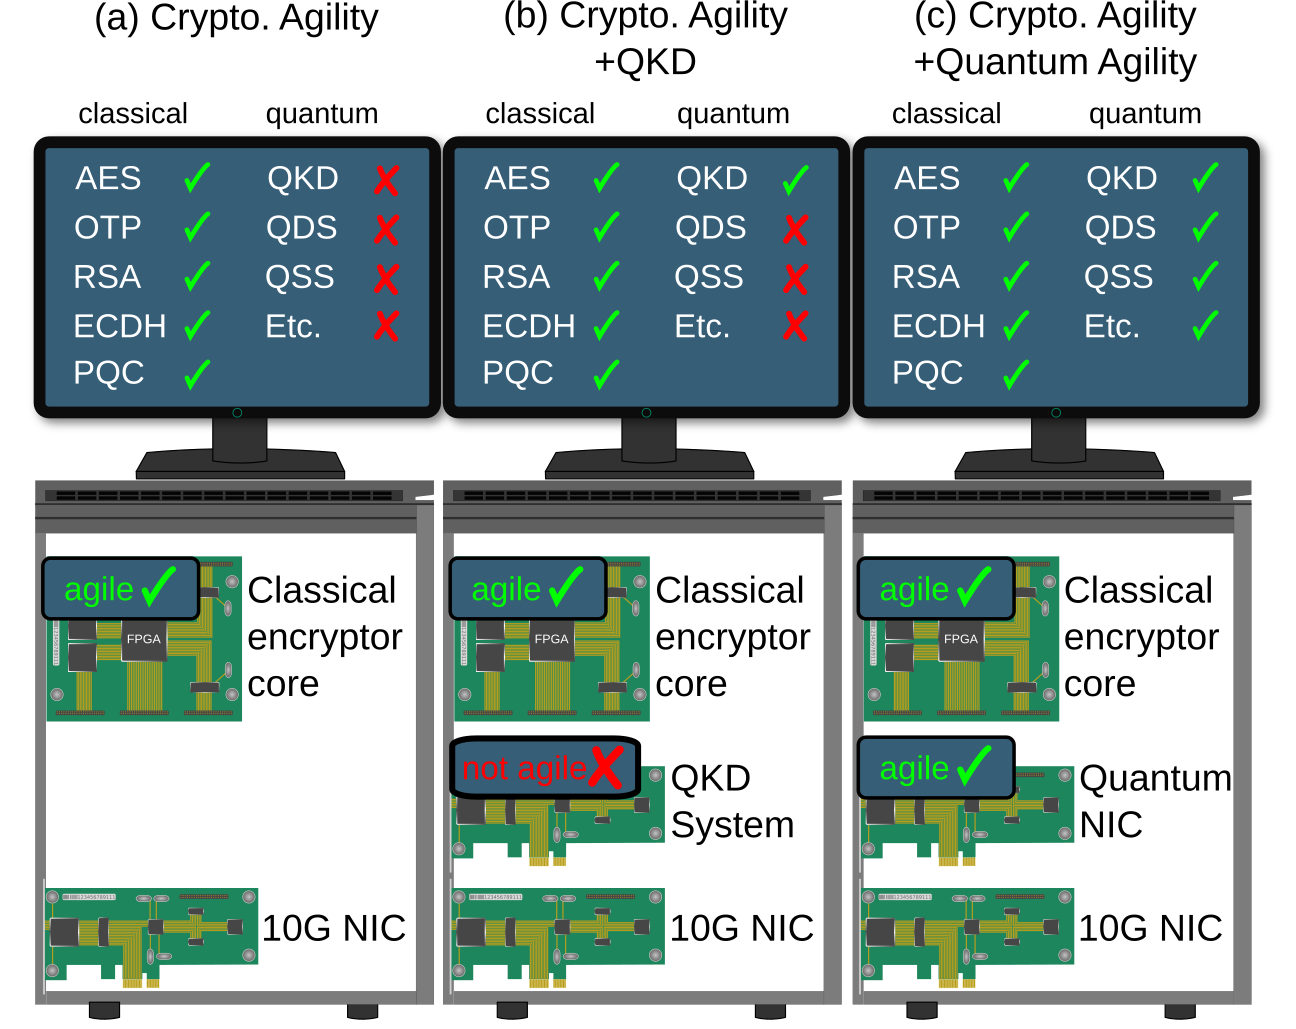
\includegraphics[draft=false]{aqc/Fig1-qagility}
\caption{\label{fig:agility} An agile cryptographic system involves a middleware which interacts between the user and the underlying crypto-core. The crypto-core (algorithm) may be readily replaced without affecting the rest of the software architecture. (a) Currently implemented classical crypto-agility. (b) QKD-assisted crypto-agility, in which several classical protocols may be run over secure channels first encrypted via a QKD link. (c) Full quantum crypto-agility which can choose interchangably between many different quantum protocols. A so-called Quantum Network Inferface Card (NIC) is used to send and receive quantum states. Classical algorithms and quantum algorithms can be replaced as necessary. The classical protocols displayed are: Advanced Encryption Standard (AES), One-time Pad (OTP), Rivest-Shamir-Adleman (RSA), Elliptic-Curve Diffie-Hellman (ECDH) and post-quantum cryptography (PQC). \emph{Picture credit: Stefan Richter in Ref.~\cite{Richter2020}}}
\end{figure}


The framework of crypto-agility seems ideal to help us answer Q1 and Q2. It is natural to separate the application layer (the task to be performed) from the underlying algorithm (which we may call a "quantum crypto-core"). One might even envisage a future library of quantum security software, in which one can select between the appropriate underlying algorithm based on the desired task and the available network hardware. We are then motivated to explore the quantum analogue of classical crypto-agility as a step towards efficient and flexible quantum communications networks.



There are two potential ways to translate the idea of classical crypto-agility into the quantum realm. We depict them both in Figs.~\ref{fig:agility}b,~\ref{fig:agility}c. The first we refer to as ``QKD-assisted crypto agility'', which may be seen as a generalization of the unconditionally secure classical secret sharing protocols, Sec.~\ref{sec:qss_qcss}, and signatures protocols \cite{Wallden2015, Amiri2016a} which implicitly require QKD first in order to remain secure. In this approach, a QKD system delivers fresh secure random keys which may be used for many different protocols. This is the stance taken by the ETSI QKD ISG $004$ \cite{ETSI004} and $014$ \cite{ETSI014} standardization efforts, which specify interface design between a QKD system (hardware) and the key management system (software). We expect that this QKD-assisted crypto agility will form an important cornerstone for future quantum networks. %This viewpoint on agility is displayed in Fig.~\ref{fig:agility}~(b).

However, as was shown in Ref.~\cite{Amiri2016} in the context of QDS, it is not always optimal to perform QKD and then a classical protocol. There may be channels over which QKD is not possible, or hardware setups over which the costly reconciliation procedures are difficult. The second viewpoint of quantum crypto-agility may thus be referred to as a ``fully quantum crypto agility,'' Fig.~\ref{fig:agility}c. Rather than building upon an underlying and fixed QKD system, such a setup should have the capability to perform multiple quantum communication protocols. This should use the so-called \emph{quantum network interface card} in Fig.~\ref{fig:agility}. This viewpoint explicitly recognises the fact that multiple quantum cryptographic protocols differ only in classical postprocessing while sharing a quantum stage and so a full QKD protocol may not be required. %In this case the choice of quantum protocol to perform is reduced simply to an update 
In a deployed system the ability to perform new quantum cryptographic protocols may then be reduced to a mere upgrade of classical firmware to control the postprocessing.


%\MT{Do I want a statement along the lines of "It is important to relaize that the transfer of the crypto-agility idea to the field of quantum cryptography changes its meaning..." from the paper?}

In Fig.~\ref{fig:big_agile} we present an example of an agile quantum communications stack which expresses the viewpoint of Fig.~\ref{fig:agility}c. The stack provides clear separation between the user (software layer) and the physical hardware layer, and may be interpreted as analogous to recent work on compilers for quantum computers \cite{Killoran2018, qiskit, Murali2019}.

%\MT{chat about this picture.}
\begin{figure}[htp]
\floatbox[{\capbeside\thisfloatsetup{capbesideposition={left,top},capbesidewidth=4cm}}]{figure}[\FBwidth]
{\caption{\label{fig:big_agile} Agile quantum communications stack following the viewpoint of Fig.~\ref{fig:agility}c. The \emph{user app} layer allows a user to select a task they wish to perform, (e.g. message encryption, message authentication, secret sharing). The agile middleware provides a separation between the user (software) and underlying quantum crypto-system (hardware). The \emph{primitive} layer selects the desired cryptographic primitive (e.g. QKD, QDS, QSS, RSA), and instructs the \emph{protocol \& hardware abstraction} layer to run the protocol via a library of known functions (e.g. ``send coherent state,'' ``perform heterodyne detection''). These commands are interpreted by the \emph{hardware} layer and sent to the physical hardware setup. The agile system should be flexible and allow for switching between different tasks, different protocols and different hardware setups. \emph{Picture credit: Stefan Richter in Ref.~\cite{Richter2020}}}}
{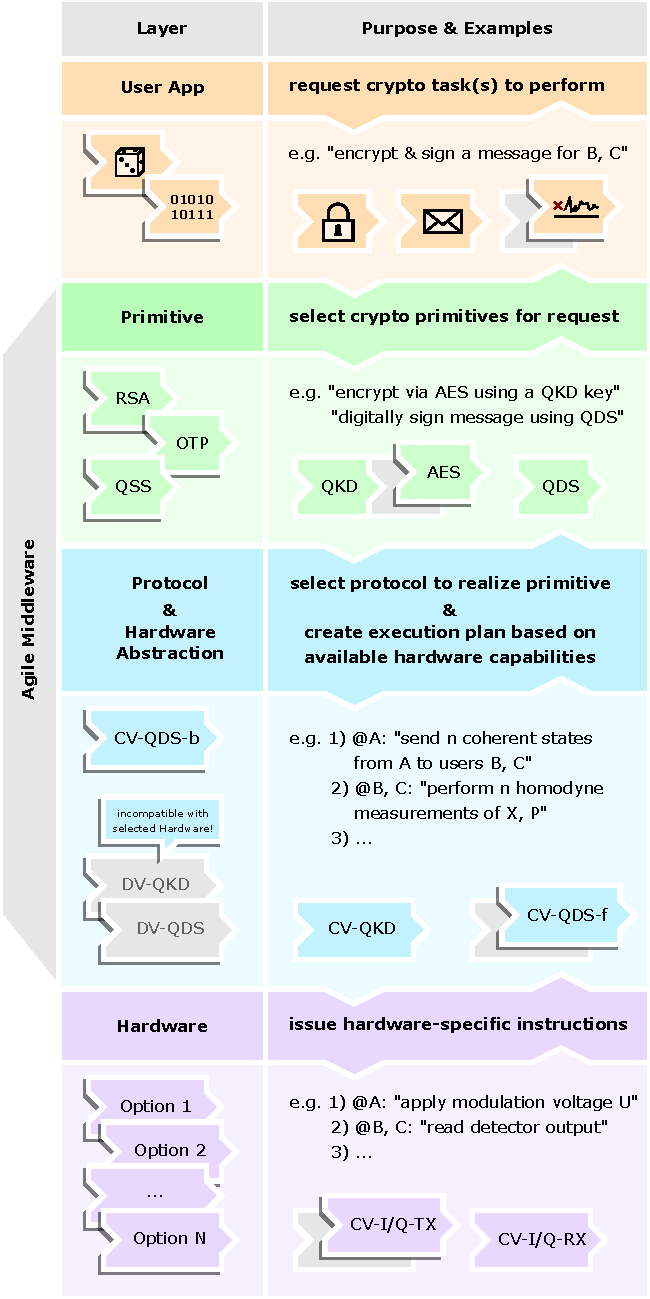
\includegraphics[draft=false, width=10cm]{aqc/layers_5}}
\end{figure}




\clearpage
\section{CV agile quantum systems}
%Make sure to acknowledge that this text is very similar to Richter2020 Section 3. Which is fine, since I wrote it and it wasn't edited by coauthors. 

To illustrate the above discussion, in this section we will introduce and analyse two quantum systems which are capable to implement multiple protocols over the same hardware setups. Within an agile system , the protocols differ only at the level of classical postprocessing. Our hardware setup is explicitly designed with question Q$2$ in mind, and with a desire for compatibility with currently deployed network architecture. The systems therefore are fully continuous-variable, and rely on distribution of phase-modulated QPSK coherent states and their heterodyne phase detection \cite{Agrawal2008}. This renders each system highly compatible with deployed telecommunications infrastructure, and paves the way to an integration between our agile systems into deployed communication links which can run with up to $100$~GHz sending rate \cite{Khan2015, Khan2016}. In Sec.~\ref{sec:aqc_experiment} we describe and analyse an experimental implementation of the agile systems discussed here.

We will consider the following tasks:

\textbf{QDS - quantum digital signatures}: allows for secure authentication of a classical message. It has been explicitly demonstrated that because of its small overhead, QDS may run over channels for which QKD is insecure \cite{Amiri2016}.

\textbf{QSS - quantum secret sharing}: allows for secure distribution of a classical secret among a conspiracy of potentially dishonest recipients.

\textbf{QKD - quantum key distribution}: allows for secure key distribution of identical randomly-generated bits between players. These keys may them be used for encryption via one-time pad \cite{Schneier1996}.

The tasks QDS and QSS are discussed in Chapters~\ref{chapter:qds},~\ref{chapter:qss} above, while the reader is referred to Refs.~\cite{Laudenbach2017, Scarani2009} for review of QKD. The tasks QDS and QSS are inherently multipartite, while QKD is inherently bipartite\footnote{Though note the existence of its multipartite generalization - quantum conferencing \cite{Ottaviani2017b, Ottaviani2019}}. In what follows we will use quantum networks with three players to allow for multipartite tasks, while also allowing for bipartite QKD to be performed.

\begin{figure}[htp]
\captionsetup{width=0.8\linewidth}
\centering
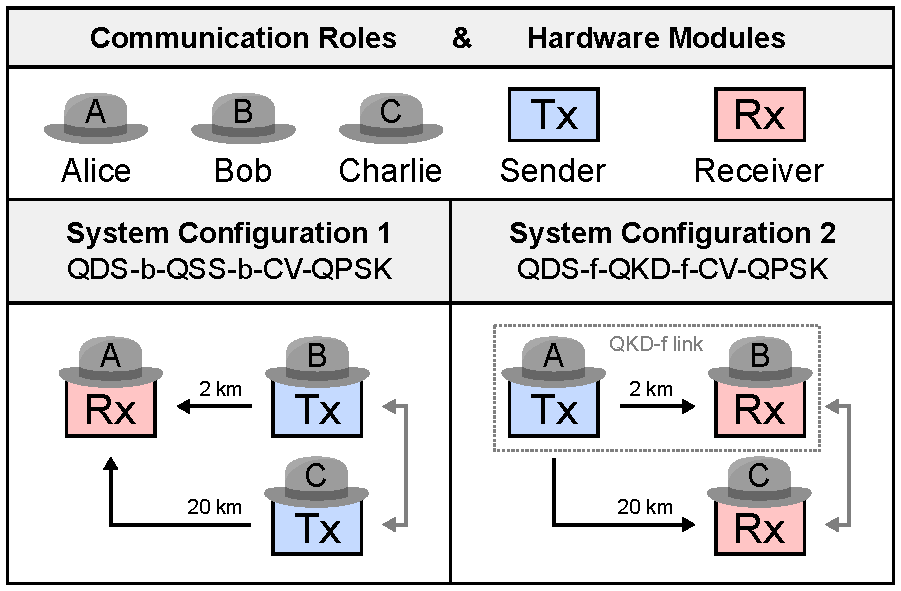
\includegraphics[draft=false, width=1.0\linewidth]{aqc/Fig2_roles-v8}
\caption{\label{fig:agile_tasks} Our two agile quantum systems. Depending on the setup configuration and the chosen task, the hardware modules (Tx, Rx) perform either as Alice or as Bob/Charlie. Tx: hardware sender module. Rx: hardware receiver modules. Hardware specifications are discussed in Sec.~\ref{sec:aqc_experiment}. \emph{Picture credit: Stefan Richter in Ref.~\cite{Richter2020}}}
\end{figure}

We therefore propose two separate agile quantum systems, one which may perform tasks QDS and QSS, and the other which may perform tasks QDS and QKD. We display these two systems in Fig.~\ref{fig:agile_tasks}. The crucial aspect is the separation between the abstract user layer defining the roles performed in the protocols, and the hardware layer. For example, the task QDS can be performed in either of the two systems, and Alice can either choose to be the sender of the quantum states or their receiver, depending on available hardware. We denote our two systems as \systemB \;and \systemF. The labels indicate which tasks are supported; the underlying quantum states which they use (QPSK alphabet), and in which direction the quantum states are exchanged ("f" - forward, Alice sends quantum states to Bob and Charlie; or "b" - backward, Bob and Charlie send quantum states to Alice). The forward- or backward- distinction can be seen as related to\footnote{but not equivalent to} direct- or reverse-reconcilition in QKD \cite{Laudenbach2017}, in which quantum and classical information flow either in the same direction or in opposite directions.




%\clearpage
\section{Agile system \systemB}\label{sec:aqc_systemb}
The first agile system we consider runs in the $b$-configuration, Fig.~\ref{fig:agile_tasks}, in which Bob and Charlie are the senders of quantum states while Alice is their receiver. We immediately see that the QSS protocol proposed and analysed in Chapter~\ref{chapter:qss} may be inherited into this agile system, c.f. Fig.~\ref{fig:qss_distribution_stage}. For consistency with notation we will now refer to this QSS protocol as QSS-$b$, and we will analyse it further below in Sec.~\ref{sec:aqc_qssb}.

We also propose a second cryptographic protocol which fits into the system \systemB, which performs the QDS task. We refer to the second protocol as QDS-$b$, and will analyse it below in Sec.~\ref{sec:aqc_qdsb}. Unlike the QDS protocol analysed in Chapter~\ref{chapter:qds}, for QDS-$b$ it is Bob and Charlie who are the senders of quantum states, while Alice is the recipient. %We will describe the protocol below, and then discuss how its security analysis must differ from Chapter~\MT{X}, and demonstrate how it fulfils QDS requirements $1-5$ from Chapter~\MT{X}.
Our first agile system \systemB \; is thus able to perform both QSS and QDS tasks using identical quantum resources. %\MT{Say somewhere my nice line about the quantum stage being "agnostic" to final protocol}

\subsection{Protocol QDS-$b$}

%\MT{I can have a picture about the QDS-b implementation.}

\begin{figure}[htp]
\captionsetup{width=0.8\linewidth}
\centering
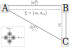
\includegraphics[width=0.8\linewidth, draft=false]{aqc/qdsb_setup}
\caption{\label{fig:qdsb_setup} Setup of protocol QDS-$b$. Alice (A) wishes to securely sign a $1$~bit message $m$. Bob and Charlie distributes quantum coherent states $\ket{\phi_j^{\left(B, C\right)}}$ to Alice along insecure quantum distribution channels (solid lines) during the Distribution stage. Bob and Charlie swap elements of their classical signatures elements via a securely encrypted classical channel (dotted lines). During the Messaging stage Alice sends $\Sigma$, containing her message $m$ and her corresponding eliminated signature $\sigma_m$ along a classical broadcast channel (dot-dashed line). Inset: QPSK alphabet.}
\end{figure}

Recall that a QDS scheme must fulfill the requirements from List~\ref{list:qds_requirements} and provide security against a dishonest forger, security against repudiation, and should be robust and succeed when all parties behave honestly, Fig.~\ref{fig:qds_attacks}. We will first outline how protocol QDS-$b$ runs, and then prove that it fulfills each of these requirements.

The protocol QDS-$b$ runs as follows:
%\MT{Make sure it written analogously to QDS-$f$ above.}

\subsubsection*{Distribution stage}

\paragraph{Step $1$.}
For each future message $m \in \left\{0, 1\right\}$ which Alice wishes to securely sign, Bob and Charlie create the classical strings
\begin{equation}
\Phi_m^{\left(B, C\right)} = \left\{\phi_{j, m}^{\left(B, C\right)}\right\}_{j=1}^L
\end{equation}
of length $L$, where the $\phi_j$ are complex phases chosen from the QPSK alphabet. The $\phi_j$ are assumed to be chosen uniformly at random.
%Bob and Charlie both send Alice a sequence, length $L$, of coherent states chosen randomly from the QPSK alphabet. Bob and Charlie each keep a record of which states they have sent.


\paragraph{Step $2$.} Bob and Charlie form sequences of quantum coherent states corresponding to elements of $\Phi_m^{\left(B, C\right)}$ and distribute them through the quantum channels to Alice. Bob and Charlie each keep a record of $\Phi_m^{\left(B, C\right)}$.

\paragraph{Step $3$.} Alice performs heterodyne detection on each received state and receives phase outcomes which we denote $x_{B, C} = \qout + i \pout$, with the subscript denoting which player sent the coherent state. Since measurement is performed immediately on receipt of the state, Alice does not require quantum memory and the remainder of the protocol is entirely classical. Bob and Charlie will each send different sequences of coherent states, which allows security against forgery.

At the end of the quantum stage of the protocol, Alice possesses two classical strings, each of length $L$, which contain her complex phase measurements. She now forms eliminated signatures $A_{B, C}^m$ by writing down which two states from the QPSK alphabet are least-compatible with Alice's measurement. The eliminated signatures are formed identically to Fig.~\ref{fig:qds_mismatches}.

\paragraph{Step $4$. \emph{Symmetrization:}} Bob and Charlie swap a random half of their $\Phi_m^{\left(B, C\right)}$ in order to guard against a dishonest Alice. Bob (Charlie) now possesses signature $X_B^m, \left(X_C^m\right)$ which consists of two halves of length $L/2$, one of which was generated by Bob (Charlie), and one of which was received during the swapping. We denote the first half by $Y_m^{\left(B\right)}$ and the second half by $Z_m^{\left(B\right)}$ in analogy with Chapter~\ref{chapter:qds}, and similarly for Charlie. Contrary to Chapter~\ref{chapter:qds}, strings $Y_m^{\left(B\right)}$ and $Z_m^{\left(B\right)}$ contain phase information, while $A_{B, C}^m$ are eliminated signatures. This swapping step will ensure security against repudiation.

\subsubsection{Messaging stage}
Messaging may occur any time after distribution.

\paragraph{Step $5$.} Alice sends the classical information $\Sigma = \left(m, \sigma_m\right)$ to Bob. The $m$ is the message she would like to convey, and her signature is $\sigma_m = \left(A_B^m, A_C^m\right)$. 

\paragraph{Step $6$.} Bob rearranges $\sigma_m \rightarrow \tilde{\sigma}_m := \left(\tilde{A}_{Y, m}^B, \tilde{A}_{Z, m}^B\right)$ by selecting elements from Alice's declaration which correspond to the two halves of his signature. Bob compares $\tilde{\sigma}_m$ to his two halves and counts the number of mismatches. Message $m$ is accepted as genuine provided that
\begin{equation}
\mathcal{M}\left(Y_m^B, \tilde{A}_{Y, m}^B\right) \le s_B \frac{L}{2} \qq{and} \mathcal{M}\left(Z_m^B, \tilde{A}_{Z, m}^B\right) \le s_B \frac{L}{2}
\end{equation}
otherwise the protocol aborts. %The threshold $s_B$ in general takes a different value from the $s_B$ used in Chapter~\ref{chapter:qds}.

\paragraph{Step $7$.} If Bob has accepted $m$ then he forwards $\Sigma$ to Charlie, who similarly checks for mismatches between Alice's eliminated signature and his signature. Charlie accepts the message if
\begin{equation}
\mathcal{M}\left(Y_m^C, \tilde{A}_{Y, m}^C\right) \le s_C \frac{L}{2} \qq{and} \mathcal{M}\left(Z_m^C, \tilde{A}_{Z, m}^C\right) \le s_C \frac{L}{2}
\end{equation}
otherwise it aborts. %The $s_C$ in general takes a different value from the $s_C$ in Chapter~\ref{chapter:qds}. 
If both Bob and Charlie accept $m$ then the protocol has succeeded. 

It is worth noting some important similarities and differences between QDS-$b$ and the protocol described in Ch.~\ref{chapter:qds}. While both protocols rely on QPSK alphabet, heterodyne detection, and the construction and comparison of eliminated signatures, the security analysis required for the two protocols differs. Crucially, while in Ch.~\ref{chapter:qds} the $j^{\text{th}}$ element of a dishonest forger's declaration is a single phase chosen from QPSK, for QDS-$b$ he must effectively declare \emph{two} phases from QPSK in the form of an eliminated signature element. Additionally, while QDS in Ch.~\ref{chapter:qds} shares similarities with reverse-reconciliation QKD since a forging Bob had to guess Charlie's measurement outcomes, here QDS-$b$ shares similarities with direct-reconciliation QKD as a forging Bob will have to guess Charlie's sent state. We will later see how this affects performance of the protocol. 

\subsection{QDS-$b$ security}
Let us consider the security of QDS-$b$ and check how it fulfils the requirements for a QDS protocol. 

\subsubsection{Security against repudiation}
Recall that during a repudiation attack Alice will try to force Bob and Charlie to disagree about whether her message is genuine. Proof of security against repudiation follows identical lines to Sec.~\ref{sec:qds_security_repudiation}.

We assume that Alice is free to manipulate her declared $A_{B, C}^m$ and she has full control over the mismatch rates $p_B \left(p_C\right)$ with respect to states she originally received from Bob and Charlie. Alice may even choose $p_B$ or $p_C$ to be zero. Security against repudiation arises from the Symmetrizaton step of the protocol. After Bob and Charlie have swapped classical information, they each possess two half-signatures, length $L/2$, consisting either of information which they held originally or which they received during swapping. Alice succeeds in her repudiation attack if Bob accepts both of his halves as genuine while Charlie rejects at least one of his halves as fake. Therefore the probability of successful repudiation is given by

\begin{equation}
\varepsilon_{\text{repudiation}} = \text{P}\left[\left(E_A \cap E_B\right) \cap \left(E_C \cup E_D\right) \right]
\end{equation}

\noindent where the events $E_A, E_B, E_C, E_D$ are defined as

\begin{align}
&\mathcal{M}\left(Y_m^B, \tilde{A}_{Y, m}^B\right) \le s_B \frac{L}{2}, \notag \\
%
&\mathcal{M}\left(Z_m^B, \tilde{A}_{Z, m}^B\right) \le s_B \frac{L}{2}, \notag \\
%
&\mathcal{M}\left(Y_m^C, \tilde{A}_{Y, m}^C\right) > s_C \frac{L}{2}, \qq{and}\notag \\
%
&\mathcal{M}\left(Z_m^C, \tilde{A}_{Z, m}^C\right) > s_C \frac{L}{2},
\end{align}
respectively.

Applying probability inequalities Eq.~\ref{eqn:prob_inequality_1},~\ref{eqn:prob_inequality_2} and Hoeffding's inequalities Eq.~\ref{eqn:hoeffding1},~\ref{eqn:hoeffding2}, following the analysis from Sec.~\ref{sec:qds_security_repudiation} we see that

\begin{equation}
\varepsilon_{\text{repudiation}} \le \text{min}\left\{ 2 \; \exp\left(-\left[ p - s_B\right]^2 L\right), 2 \; \exp\left( - \left[ s_C - p\right]^2 L\right) \right\}
\end{equation}
\noindent 
provided that $s_B \le s_C$. The probability $\varepsilon_{\text{repudiation}}$ is maximized when
\begin{equation}
p = \frac{s_B + s_C}{2}.
\end{equation}

\noindent Finally we arrive at,
\begin{equation}\label{eqn:aqc_repudiation}
\varepsilon_{\text{repudiation}} \le 2 \; \exp\left( - \frac{\left[s_C - s_B\right]^2}{4}L\right)
\end{equation}

\noindent identically to Ch.~\ref{chapter:qds}. We have seen that repudiation is only affected by the relative mismatch rates between players' signatures and not by who actually possesses the signatures. This is perhaps unsurprising, since in both QDS protocols it is assumed that Alice has complete control over mismatch rates with respect to states held by players before swapping.

\subsection{Robustness}
The robustness of the protocol depends only on parameters $s_B$ and $\perr$. Using Hoeffding inequality Eq.~\ref{eqn:qds_hoeffding2} identically to Sec.~\ref{sec:qds_security_robustness} we may derive 
\begin{equation}\label{eqn:aqc_robustness}
\varepsilon_{\text{honest abort}} \le 2 \, \exp\left( - \left[s_B - \perr\right]^2 L\right)
\end{equation}
provided that $\perr \le s_B$. The probability $\perr$ of honest mismatch may be modelled as in Sec.~\ref{sec:qds_modelling_perr} and does not change here.

\subsection{Security against forgery}
Since Bob already knows half of Charlie's signature elements (those which Bob himself forwarded) and since $s_B \le s_C$ the most dangerous forger is a dishonest Bob. He is therefore assumed to be the eavesdropper on Charlie's distribution of quantum states, and tries to gain information about the $L/2$ signature elements which Charlie generated himself.

Using Hoeffding's inequalities Eq.~\ref{eqn:qds_hoeffding1} as in Sec.~\ref{sec:qds_security_forgery} we see that at a forging attack succeeds with probability 
\begin{equation}\label{eqn:aqc_forgery}
\varepsilon_{\text{forgery}} \le 2 \; \exp\left( - \left[ \pe - s_C\right]^2 \frac{L}{2} \right)
\end{equation}
provided that $\pe \ge s_C$. 

\subsection{Bounding $\pe$}
All that remains is to bound $\pe$. This will expose several of the differences between QDS-$b$ and QDS from Chapter~\ref{chapter:qds}.

%\MT{I am just copying and pasting the following from Richter2020. Which is fine because I wrote it and it hasn't been edited.}

Consider the $j^\text{th}$ signature element. Charlie holds some $c_j$ denoting which state from the QPSK alphabet he sent. During Messaging, Bob will declare an eliminated signature element, $B_j = \left\{b_j^1, b_j^2\right\}$ which is chosen to minimize $\pe$ and should be the outcome of some optimal strategy on his system, denoted $\mathbb{B}$. The $b_j^1, b_j^2$ correspond to adjacent elements of the QPSK alphabet, with a mismatch occurring if $b_j^1 = c_j$ or $b_j^2 = c_j$. %Additionally, we assume that $B_j$ is the result of some optimal strategy involving Bob's quantum system, $\mathbb{B}_j$.

We define an error variable $\mathcal{E}$ such that 

\begin{equation*}\label{eqn:error}
\mathcal{E}_j = 
\begin{cases}
1 & \text{if a mismatch occurs between $\mathcal{F}_j$ and $\mathcal{G}_j$} \\
0 & \text{otherwise}
\end{cases}
\end{equation*}
which measures whether a mismatch has occurred between $\mathcal{F}_j$ and $\mathcal{G}_j$. Then $\pe \equiv \text{P}\left(\mathcal{E}_j = 1\right)$, and the Shannon entropy $\text{H}\left(\mathcal{E}_j\right) = \text{h}\left(\pe\right)$ is the binary entropy, since $\left|\mathcal{E}_j\right| = 2$. 

Now, consider the conditional entropy $\text{H}\left(\mathcal{E}_j, b_j^1, b_j^2 \given c_j\right)$. Via the chain rule for conditional entropies,

\begin{equation*}
\text{H}\left(\mathcal{E}_j, b_j^1, b_j^2 \given c_j\right) = \text{H}\left(b_j^1, b_j^2 \given c_j\right)
\end{equation*}

\noindent where we have used the fact that once $b_j^1, b_j^2$ and $c_j$ are known, $\mathcal{E}_j$ is uniquely determined. Using the chain rule on $\text{H}\left(\mathcal{E}_j, b_j^1, b_j^2 \given c_j\right)$ again, but for a different variable, we get

\begin{align*}
\text{H}\left(\mathcal{E}_j, b_j^1, b_j^2 \given c_j\right) &= \text{H}\left(b_j^1, b_j^2 \given \mathcal{E}_j, c_j\right) + \text{H}\left(\mathcal{E}_j \given c_j\right) \notag \\
&\le \text{H}\left(b_j^1, b_j^2 \given \mathcal{E}_j, c_j\right) + \text{h}\left(\pe\right)
\end{align*}

\noindent since conditioning can never increase entropy. Therefore, by expanding the variable $\mathcal{E}_j$,

\begin{align*}
\text{H}\left(b_j^1, b_j^2 \given c_j\right) \le \left(1 - p_e\right) &\text{H}\left(b_j^1, b_j^2 \given \mathcal{E}_j = 0, c_j\right) \\ + &\pe \; \text{H}\left(b_j^1, b_j^2 \given \mathcal{E}_j=1, c_j\right) + \text{h}\left(\pe\right).
\end{align*}

\noindent Now, $\text{H}\left(b_j^1, b_j^2 \given \mathcal{E}_j=0, c_j\right) \le \log_2\left(2\right) = 1$, and similarly for $\mathcal{E}_j=1$, and so

\begin{equation}\label{eqn:A7}
\text{H}\left(b_j^1, b_j^2 \given c_j\right) \le 1 + \text{h}\left(p_e\right).
\end{equation}

\noindent Finally, we expand the conditional entropy in terms of the joint entropy and the mutual information,

\begin{align}\label{eqn:A8}
\text{H}\left(b_j^1, b_j^2 \given c_j\right) &= \text{H}\left(b_j^1, b_j^2\right) - \text{I}\left(b_j^1, b_j^2 : c_j\right) \notag \\
&\ge 2 - \chi\left(b_j^1, b_j^2 : c_j\right)
\end{align}

\noindent where we have used the fact that \emph{a priori} there are four choices for the pair $b_j^1, b_j^2$, and where $\chi$ is the Holevo information. Combining Eqs.~\ref{eqn:A7},~\ref{eqn:A8} we arrive at

\begin{equation}
\text{h}\left(\pe\right) \ge 1 - \chi\left(b_j^1, b_j^2 : c_j\right).
\end{equation}

\noindent Surprisingly this equation has similar form to Eq.~\ref{eqn:qds_hpe}, but with a Holevo information calculated differently, as shown below. %TODO: add a comment about how the Holevo information here is different.


Once $\pe$ and $\perr$ are bounded for the protocol, the probability $\varepsilon_{fail}$ that the protocol fails can be found. For concreteness, we assign equal probability to the failure of the protocol either by allowing a forging or repudiation attack, or by aborting when all players are honest, that is

\begin{equation*}
\varepsilon_{\text{fail}} = \varepsilon_{\text{honest abort}} = \varepsilon_{\text{repudiation}} = \varepsilon_{\text{forgery}},
\end{equation*}

\noindent and by choosing $s_B = p_{err} + \left(p_e + p_{err}\right)/4$; $s_C = p_{err} = 3\left(p_e - p_{err}\right)/4$, in order to satisfy the second two equalities, we arrive at 

\begin{equation}\label{eqn:aqc_qdsb_efail}
\varepsilon_{fail} \le 2 \exp \left[ - \frac{\left( p_e - p_{err} \right)^2}{16} L \right]
\end{equation}

\noindent when $\perr< s_B < s_C < \pe$.

\subsubsection{Calculating Holevo}

Finally, we note that under a beamsplitter attack BS$0$ Bob's \emph{a priori} state is
\begin{equation}\label{eqn:qdsb_apriori_state}
\rho_B = \frac{1}{4}\sum_{k=0}^3 |\sqrt{1-T}\alpha_k\rangle\langle\sqrt{1-T}\alpha_k|
\end{equation}
when states $|\alpha_k\rangle$ from the QPSK alphabet are sent through lossy channel with transmission T. Bob's \emph{a posteriori} state is simply $\rho_{B}^k = |\sqrt{1-T}\alpha_k\rangle\langle \sqrt{1-T}\alpha_k|$, from which his Holevo information is calculated as

\begin{equation}
\chi = S\left(\rho_B\right) - \sum_{k=0}^3 p\left(k\right) S\left(\rho_E^k\right)
\end{equation}
with $S$ the Von Neumann entropy. Under attack BS$0$ state $\rho_B^k$ is pure and so $\chi = S\left(\rho_B\right)$. Other attacks may be readily considered, and we present the requisite states in Sec.~\ref{appendix:qdsb_states}. \MT{do this.} Bob's mismatch rate $\pe$ may now be calculated and we obtain figure of merit signature length $L$ via Eq.~\ref{eqn:aqc_qdsb_efail}.



\subsection{QDS-$b$ postselection}
Let us apply the postselection technique described in Sec.~\ref{sec:qds_postselection} to protocol QDS-$b$. We shall see that while previously postselection was mainly used to improve efficiency of the protocol over parameters in which it was already secure, here it is absolutely necessary in order to sign a message for even short distances. We define the region $\rps\left(\Delta_r, \Delta_\theta\right)$, as in Fig.~\ref{fig:rps}, and allow honest recipients to only accept $x \in \mathbb{C} \setminus \rps$. 

The crucial quantity to consider is $g_{\text{sec}} := \pe - \perr$, measuring the advantage which and honest player has over a dishonest one. The protocol is secure provided that $g_{\text{sec}} > 0$, Eq.~\ref{eqn:aqc_qdsb_efail}. For protocol QDS-$b$, the probability $\pe$ does not depend on Alice's heterodyne measurement, since a dishonest player attacks the sender of the quantum states. Therefore, $\pe$ is unaffected by postselection.

Probability $\perr$ on the other hand is strongly affected by our choice of $\rps$. Given the probability $\text{P}\left(r e^{i \theta} \given \alpha, T\right)$ to obtain complex outcome $r e^{i \theta}$ when state $\ket{\alpha}$ is sent through a noiseless channel with transmission $T$, we see that when no postselection is used
\begin{equation}
\perr = \int\limits_{r=0}^\infty \mathrm{d}r \; r \int\limits_{\theta = \pi/2}^{3\pi/2} \mathrm{d}\theta \; \text{P}\left(r e^{i \theta} \given \alpha, T\right).
\end{equation}

\noindent Incorporating the postselection technique here corresponds to changing the limits of integration, and so when postselection is used we have

\begin{align}
\perr\left(\Delta_r, \Delta_\theta\right) = \frac{1}{\mathcal{N}} \int\limits_{r = \Delta_r}^\infty \mathrm{d}r\; r  &\left[ \int\limits_{\theta = \pi/2 + \Delta_\theta}^{\pi - \Delta_\theta} \mathrm{d}\theta \; \text{P}\left(r e^{i \theta} \given \alpha, T\right)\right. \notag \\
%
&\left. + \int\limits_{\theta = \pi + \Delta_\theta}^{3\pi/2 - \Delta_\theta} \mathrm{d}\theta \text{P}\left(r e^{i \theta}\given \alpha, T\right)\right].
\end{align}

\noindent Finally, we note that just as in Sec.~\ref{sec:qds_postselection}, we must rescale our figure of merit to
\begin{equation}
\tilde{L} = \frac{L}{\mathcal{N}},
\end{equation}
where normalization factor $\mathcal{N}$ is calculated in the usual way. Since $\tilde{L}$ (with postselection) is directly comparable to $L$ (without postselection) as a figure of merit, in the remainder of this chapter we will not distinguish between the two. However, it must always be understood that if postselection has been used then we are implicitly dealing with $\tilde{L}$.





\subsection{QDS-$b$ performance}

We plot signature length as it varies with $T$ under protocol QDS-$b$ in Fig.~\ref{fig:aqc_qdsb_lengths}. At each $T$ we have optimized over coherent state amplitude $\alpha$ and postselection parameter\footnote{As in Ch.~\ref{chapter:qds}, $\Delta_\theta>0$ worsened performance.} $\Delta_r$, and the resulting signature lengths are displayed as the solid lines in Fig.~\ref{fig:aqc_qdsb_lengths}. Black: BS$0$ attack, Red: EC attack with constant $\bar{n}=0.02$. Non-solid lines are specific choices of $\alpha$ which are close to optimal only at specific $T$. We see that choosing an $\alpha$ which is not optimal for a given channel transmission can drastically affect the signature length, and for some transmissions can even result in an increase similar to allowing a different class of attack. Since in a practical realization of the protocol, $\Delta_r$ may feasibly be chosen after the distribution of quantum states, we have optimized over $\Delta_r$ at each point in the figure.

\begin{figure}[htp]
\captionsetup{width=0.8\linewidth}
\centering
\includegraphics[draft=false, width=0.6\linewidth]{aqc/QDSb_optimal_L}
\caption{\label{fig:aqc_qdsb_lengths} QDS-$b$ signature lengths. Black: BS$0$ attack. Red: EC attack with constant $\bar{n} = 0.02$. Green, dashed: $BS0$ attack with $\alpha=0.5$. Orange, dotted: $BS0$ attack with $\alpha=0.7$, Blue, dot-dashed: EC attack with constant $\bar{n}=0.02$, $\alpha=0.5$. All lines have optimal $\Delta_r$ chosen at each point. Solid lines: optimal choice of $\alpha$ and $\Delta_r$ at each point.}
\end{figure}

To summarise, our first agile system, \systemB, is capable of performing the secure tasks QDS and QSS. We have incorporated the QSS protocol discussed in Ch.~\ref{chapter:qss} and labelled it QSS-$b$, for consistency of notation. The new protocol QDS-$b$ may be viewed as a direct-reconciliation analogue of the QDS protocol discussed in Ch.~\ref{chapter:qds}. We will implement each protocol and discuss performance in Sec.~\ref{sec:aqc_performance}.

\section{Agile system \systemF}\label{sec:aqc_systemf}

In addition to the first agile system described above, which is capable of performing both QDS and QSS tasks, we here introduce and demonstrate a second agile system, \systemF, which runs in the $f$-configuration Fig.~\ref{fig:agile_tasks}. Here, Alice is the sender of quantum states, while Bob and Charlie are the recipients. This system is capable of performing both QDS and QKD tasks.

The QKD protocol contained in \systemF \; already exists in the literature \cite{Leverrier2011a, Papanastasiou2018} and has been an active direction of research for many years. Its inclusion here illustrates that pre-existing protocols may be interpreted through an agile lens. We denote the QKD protocol QKD-$f$. The QDS protocol in $f$-configuration was analysed above in Chapter~\ref{chapter:qds}, and here we rename it as QDS-$f$.

Let us briefly consider each protocol in turn.

\subsection{Protocol QDS-$f$}
We bring the QDS protocol considered in Chapter~\ref{chapter:qds} into the system \systemF. The protocol QDS-$f$ requires no modification to run over hardware in the $f$-configuration and so the reader is referred to Ch.~\ref{chapter:qds} for details, security proof, and performance analysis. Our earlier security analysis assumed ideal behaviour. In Sec.~\ref{sec:aqc_protocol_modifications} we relax some of these assumptions and make the protocol analysis more realistic to experimental implementation.


\subsection{Protocol QKD-$f$}
QKD using heterodyne detection of a discrete-modulated alphabet of coherent states has long been proposed and analysed, owing to its ease of implementation and high compatibility with installed telecommunications infrastructure \cite{Leverrier2011a, Papanastasiou2018, Zhao2009, Bradler2017, Ghorai2019, Lin2019}. Despite its practical ease of use, theoretical work has lagged behind other CV QKD protocols, which rely on a Gaussian modulation of coherent states. Unlike DV systems, CV systems live in an infinite dimensional Hilbert space and so many of the computational methods available for QKD with single-photons are not immediately transferable \cite{Tomamichel2012}, and unlike Gaussian-modulated CV systems, coherent states with a discrete-modulation cannot be reduced to calculations on the finite-sized covariance matrix.  %TODO: ensure that different modulations are discussed in the intro chapter.

Attempts to prove security of discete-modulated CV QKD protocols have made simplifying assumptions in either of these directions. For example, in Refs.~\cite{Leverrier2011a, Ghorai2019, Lin2019} it is assumed that since the amplitude $\alpha$ of coherent states in the chosen QPSK alphabet is small the \emph{a priori} states in the protocol are approximately Gaussian. This allows covariance-matrix based methods to be used for the analysis. This assumption is only strictly true in the limit $\alpha \rightarrow 0$, and it is as yet unproven whether an attack could exploit higher order statistical moments of the \emph{a priori} state which are not captured by the covariance matrix.

%Another direction has been to truncate the size of hilbert space \cite{Ghorai2019, Lin2019, Papanastasiou2018}. This is perhaps a reasonable approach, since one can sensibly bound the dimension of an incoming quantum state by assuming that its energy is upper-bounded

Another direction has been to truncate the size of the Hilbert space \cite{Ghorai2019, Lin2019, Papanastasiou2018}. This is perhaps a reasonable approach, since for many of the infinite-dimensional states used in the QKD protocols one can find a nearby state which lives in a large but finite-dimensional Hilbert space. This becomes increasingly true for small $\alpha$. 

A QKD protocol relying on a QPSK alphabet and heterodyne detection is analysed in Ref.~\cite{Papanastasiou2018}, and it is their analysis which we lean on in this section. 


%\begin{figure}[htp]
%\centering
%\includegraphics{aqc/qkdf_setup.png}
%\caption{\label{fig:aqc_qkdf_setup}}
%\end{figure}

Alice distributes coherent state $\ket{\alpha}$ from her QPSK alphabet through the quantum channel to Bob\footnote{Alice could also perform QKD in \systemF \; with Charlie, and the discussion follows identically.}. Assuming, for now, attack BS$0$, Bob recieves $\ket{\sqrt{1-T}\alpha}$ and performs heterodyne measurement, obtaining outcome $x$ with probability
\begin{equation}
\text{P}\left(x\given \alpha, T\right) = \frac{1}{\pi}\exp\left( - \left[ x - \sqrt{T}\alpha\right]^2\right).
\end{equation}
We denote Alice's variable containing information of which coherent state she chose by $X_A$, and Bob's variable containing his measurement outcome by $X_B$. Alice and Bob then perform a reverse-reconciliation procedure \cite{Grosshans2002, Grosshans2003, Laudenbach2017} to form a secret key.

The starting point for the analysis is the Devetak-Winter key rate formula \cite{Devetak2004} 
\begin{equation}
\kappa \ge \text{I}\left(X_A : X_B\right) - \chi\left(X_B : \mathbb{E}\right)
\end{equation}

\noindent where $\mathbb{E}$ denotes Eve's quantum system. Let us calculate each term.

\subsubsection{Mutual information I}
The mutual information I is calculated in a similar fashion to the protocol QSS-$b$ discussed in Chapter~\ref{chapter:qss}. Using Eq.~\ref{eqn:intro_mutual_information} we expand $\text{I}$ as
\begin{equation}\label{eqn:qkdf_deriv_1}
\text{I}\left(X_A : X_B\right) = \text{H}\left(X_A\right) - \text{H}\left(X_A \given X_B\right).
\end{equation}

\noindent The Shannon entropy of Alice's variable is equal to $\sum_{X_A=a} - \text{P}\left(a\right) \log \text{P}\left(a\right)$ and is equal to $2$ in the ideal case. .

We may expand the conditional entropy in Eq.~\ref{eqn:qkdf_deriv_1} as
\begin{equation}\label{eqn:qkdf_deriv_2}
\text{H}\left(X_A \given X_B\right) = \int\limits_{b \in \mathbb{C}} \Diff2 b \; \text{P}\left(X_B=b\right) \text{H}\left(X_A \given X_B=b\right)
\end{equation}
where the integration is performed over all possible outcomes $b$ which Bob can obtain. The mutual information I may then be calculated by expanding $\text{H}\left(X_A \given X_B=b\right)$ and then using Bayes's formula. 

\subsubsection{Holevo information $\chi$}
We will derive the Holevo information $\chi$ which Eve has about Bob's variable $X_B$ under attack BS$0$. Her Holevo information under other attacks may be calculated likewise, using steps from Sec.~\ref{sec:qds_attack_analysis}.

When a coherent state $\alpha_k$ is chosen uniformly at random, the two-mode output state from the channel is

\begin{equation}
\rho_{B, E} = \frac{1}{4} \sum_{\alpha_k} \left[ \dyad{\sqrt{T}\alpha_k}_B \otimes \dyad{\sqrt{1-T}\alpha_k}_E\right]
\end{equation}

\noindent and so after Bob's heterodye measurement, outcome $b \in \mathbb{C}$, Eve's conditional state is

\begin{equation}\label{eqn:qkdf_eve_conditional}
\rho_{\left. E \given b\right.} = \frac{1}{4} \frac{1}{\text{P}\left(b\right)} \sum_{\alpha_k} \text{P}\left(b \given \alpha_k, T\right) \times \dyad{\sqrt{1-T}\alpha_k}_E
\end{equation}
when $\text{P}\left(b\right) = \sum_{\alpha_k}\text{P}\left(b \given \alpha_k, T\right)$ denotes the total probability that Bob measures $b$. Eve's \emph{a posteriori} entropy is then

\begin{equation}\label{eqn:qkdf_aposteriori_entropy}
S_{\text{aposteriori}} = \int\limits_{b \in \mathbb{C}} \Diff2 b \; \text{P}\left(b\right) S\left(\rho_{\left. E \given b \right.}\right)
\end{equation}

\noindent and we note that each state $\rho_{\left.E\given b \right.}$ has in general a different entropy, so Eq.~\ref{eqn:qkdf_aposteriori_entropy} cannot be simplified further. 

Eve's \emph{a priori} entropy is
\begin{equation}\label{eqn:qkdf_apriori_entropy}
S_{\text{apriori}} = S\left[\, \int\limits_{b \in \mathbb{C}} \Diff2 b \; \text{P}\left(b\right) \rho_{\left. E \given b \right.}\right],
\end{equation}
from which the Holevo information $\chi$ may be calculated. Attacks BS$1$, BS$2$ and EC may be implemented following an identical analysis to this section. The performance of protocol QKD-$f$ is discussed at length in Ref.~\cite{Papanstasiou2018} and so we refer the reader there. 



\section{Experimental implementation}\label{sec:aqc_experiment}
%\MT{Briefly describe the experiment and what data I received. I want to make this section stuff which I \emph{didn't} do, so the next section can be stuff which I have actually done.}

An experiment which investigates the above two agile systems was performed at the Max Plank Institute for the Science of Light in Erlangen (MPL) \cite{Richter2020}, Fig.~\ref{fig:aqc_experiment}. Specifically, optical sender  and receiver modules were used to implement the four protocols which are described above. A sender module (Tx) generates and distributes phase-encoded coherent states chosen from the QPSK alphabet, while a receiver module (Rx) performs heterodyne detection of the received states' phase. Depending on the required configuration, the modules Tx, Rx are variously interpreted as playing roles of Alice or Bob/Charlie, Fig.~\ref{fig:agile_tasks}. Crucially, the hardware setup is identical for every protocol within an agile system.

\begin{figure}[htp]
\captionsetup{width=0.8\linewidth}
\centering
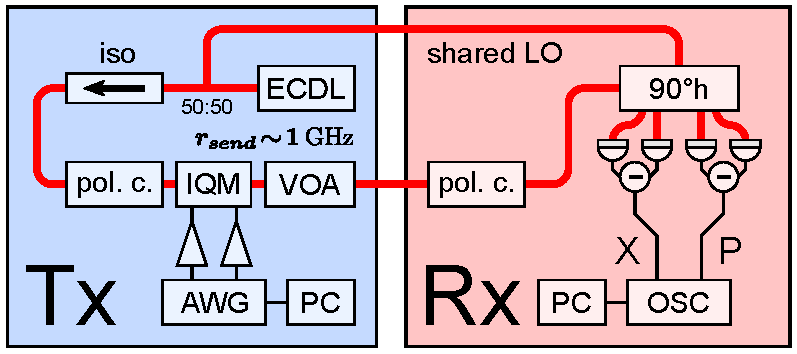
\includegraphics[draft=false, width=0.8\linewidth]{aqc/Fig2_exp-v6}
\caption{\label{fig:aqc_experiment} The sender (Tx) and receiver (Rx) modules which are used to implement each of the four cryptographic protocols considered in this Chapter. During distribution and measurement of the quantum states, hardware modules are ignorant about the roles which they are playing, and so identical experimental stages may be interpreted for different cryptographic tasks, Fig.~\ref{fig:agile_tasks}. ECDL: external-cavity diode laser; iso: isolator; VOA: variable optical attenuator; IQM: I/Q modulator; pol.c: polarization controller; AWG: arbitrary waveform generator; LO: local oscillator; $90\si{\degree}$h: $90\si{\degree}$ hybrid; OSC: oscilloscope. \emph{Picture credit: Stefan Richter in Ref.~\cite{Richter2020}}}
\end{figure}

\subsubsection{Sender module (Tx):} The sender module is depicted in Fig.~\ref{fig:aqc_experiment}. An external cavity diode laser (PurePhotonics PPCL-$300$) with a linewidth of $15$~kHz is tuned to standard telecom wavelength $1550$~nm and acts as the optical carrier. The carrier beam impinges on a $50:50$ beamsplitter which allows for a shared local oscillator (LO) between modules from one output port. From the other output port  coherent state pulses, chosen randomly from QPSK alphabet $\left\{ \ket{+ \alpha_0}, \ket{i \alpha_0}, \ket{-\alpha_0}, \ket{-i \alpha_0}\right\}$, are prepared by using an integrated I/Q modulator (Fujitsu DP-QPSK $40$~Gbps $LiNbO_3$) %\MT{I'm not sure which word "integrated" should be attached to here}. 
The I/Q modulator is driven at a rate of $1$~GHz by an arbitrary waveform generator (AWG; Keysight M$8195$A). Finally, a variable optical attenuator (VOA) attenuates the coherent states to a final amplitude of either $\alpha$ or $\alpha^\prime$, with $\alpha \le \alpha^\prime \le \alpha_0$. Coherent states with ampltude $\alpha^\prime$ will be used as phase reference states, while the signal states used for the quantum communication protocols have amplitude $\alpha$. The coherent states are then sent through the quantum channel to receiver module Rx.

\subsubsection{Receiver module (Rx):}
Module Rx interferes the received states with the shared local oscillator using the integrated Kylia COH$24$-X $90\si{\degree}$s. The two modules use a shared local oscillator which provides a frame of reference against which heterodyne phase measurement is performed using two balanced optical receivers (Discovery DSC-R$412$) with analog $3$~dB bandwidth of $20$~GHz. In principle the Tx and Rx modules do not need to share a local oscillator and bright phase-reference pulses\footnote{Though note that this may open up additional security issues \cite{Ren2019}.} could be used \cite{Huang2015}.

Outputs from the optical receivers are digitized using a digital sampling oscilloscope (Tektronix DPO$77002$SX) with a sampling rate of $25$~GS/s. Proprietary digital signal processing (DSP) algorithms are applied to the quadrature time traces. The DSP consists of a high-pass filter which eliminates low-frequency noise contributions to the signal. Finally, a phase-recovery step is performed using phase-reference states which originally had amplitude $\alpha^\prime$. %The signal states carrying quantum information which may now be used for a quantum communications task are those which originally had amplitude $\alpha$.

The Tx and Rx modules were connected by either a $2$~km or $20$~km SMF-$28$ optical fiber link which contributes to a total loss of $0.65$~dB or $4.75$~dB, respectively. This implements the realistic metropolitan distances over which the CV platform is expected to be effective. Experiments were performed for several different signal state modulation amplitudes $\alpha$. For each run of the experiment a total of $1.92\times 10^6$ states were sent in frames of $64$ which consisted of four bright reference pulses ($\alpha^\prime$) followed by $60$ signal pulses ($\alpha$). After the DSP step there remained information on $1.54 \times 10^6$ states. An example of some raw output data is displayed in Fig.~\ref{fig:aqc_experimental_trace}. The top of the figure displays raw time trace data, while the bottom displays data after the DSP.


\begin{figure}[htp]
\captionsetup{width=0.8\linewidth}
\centering
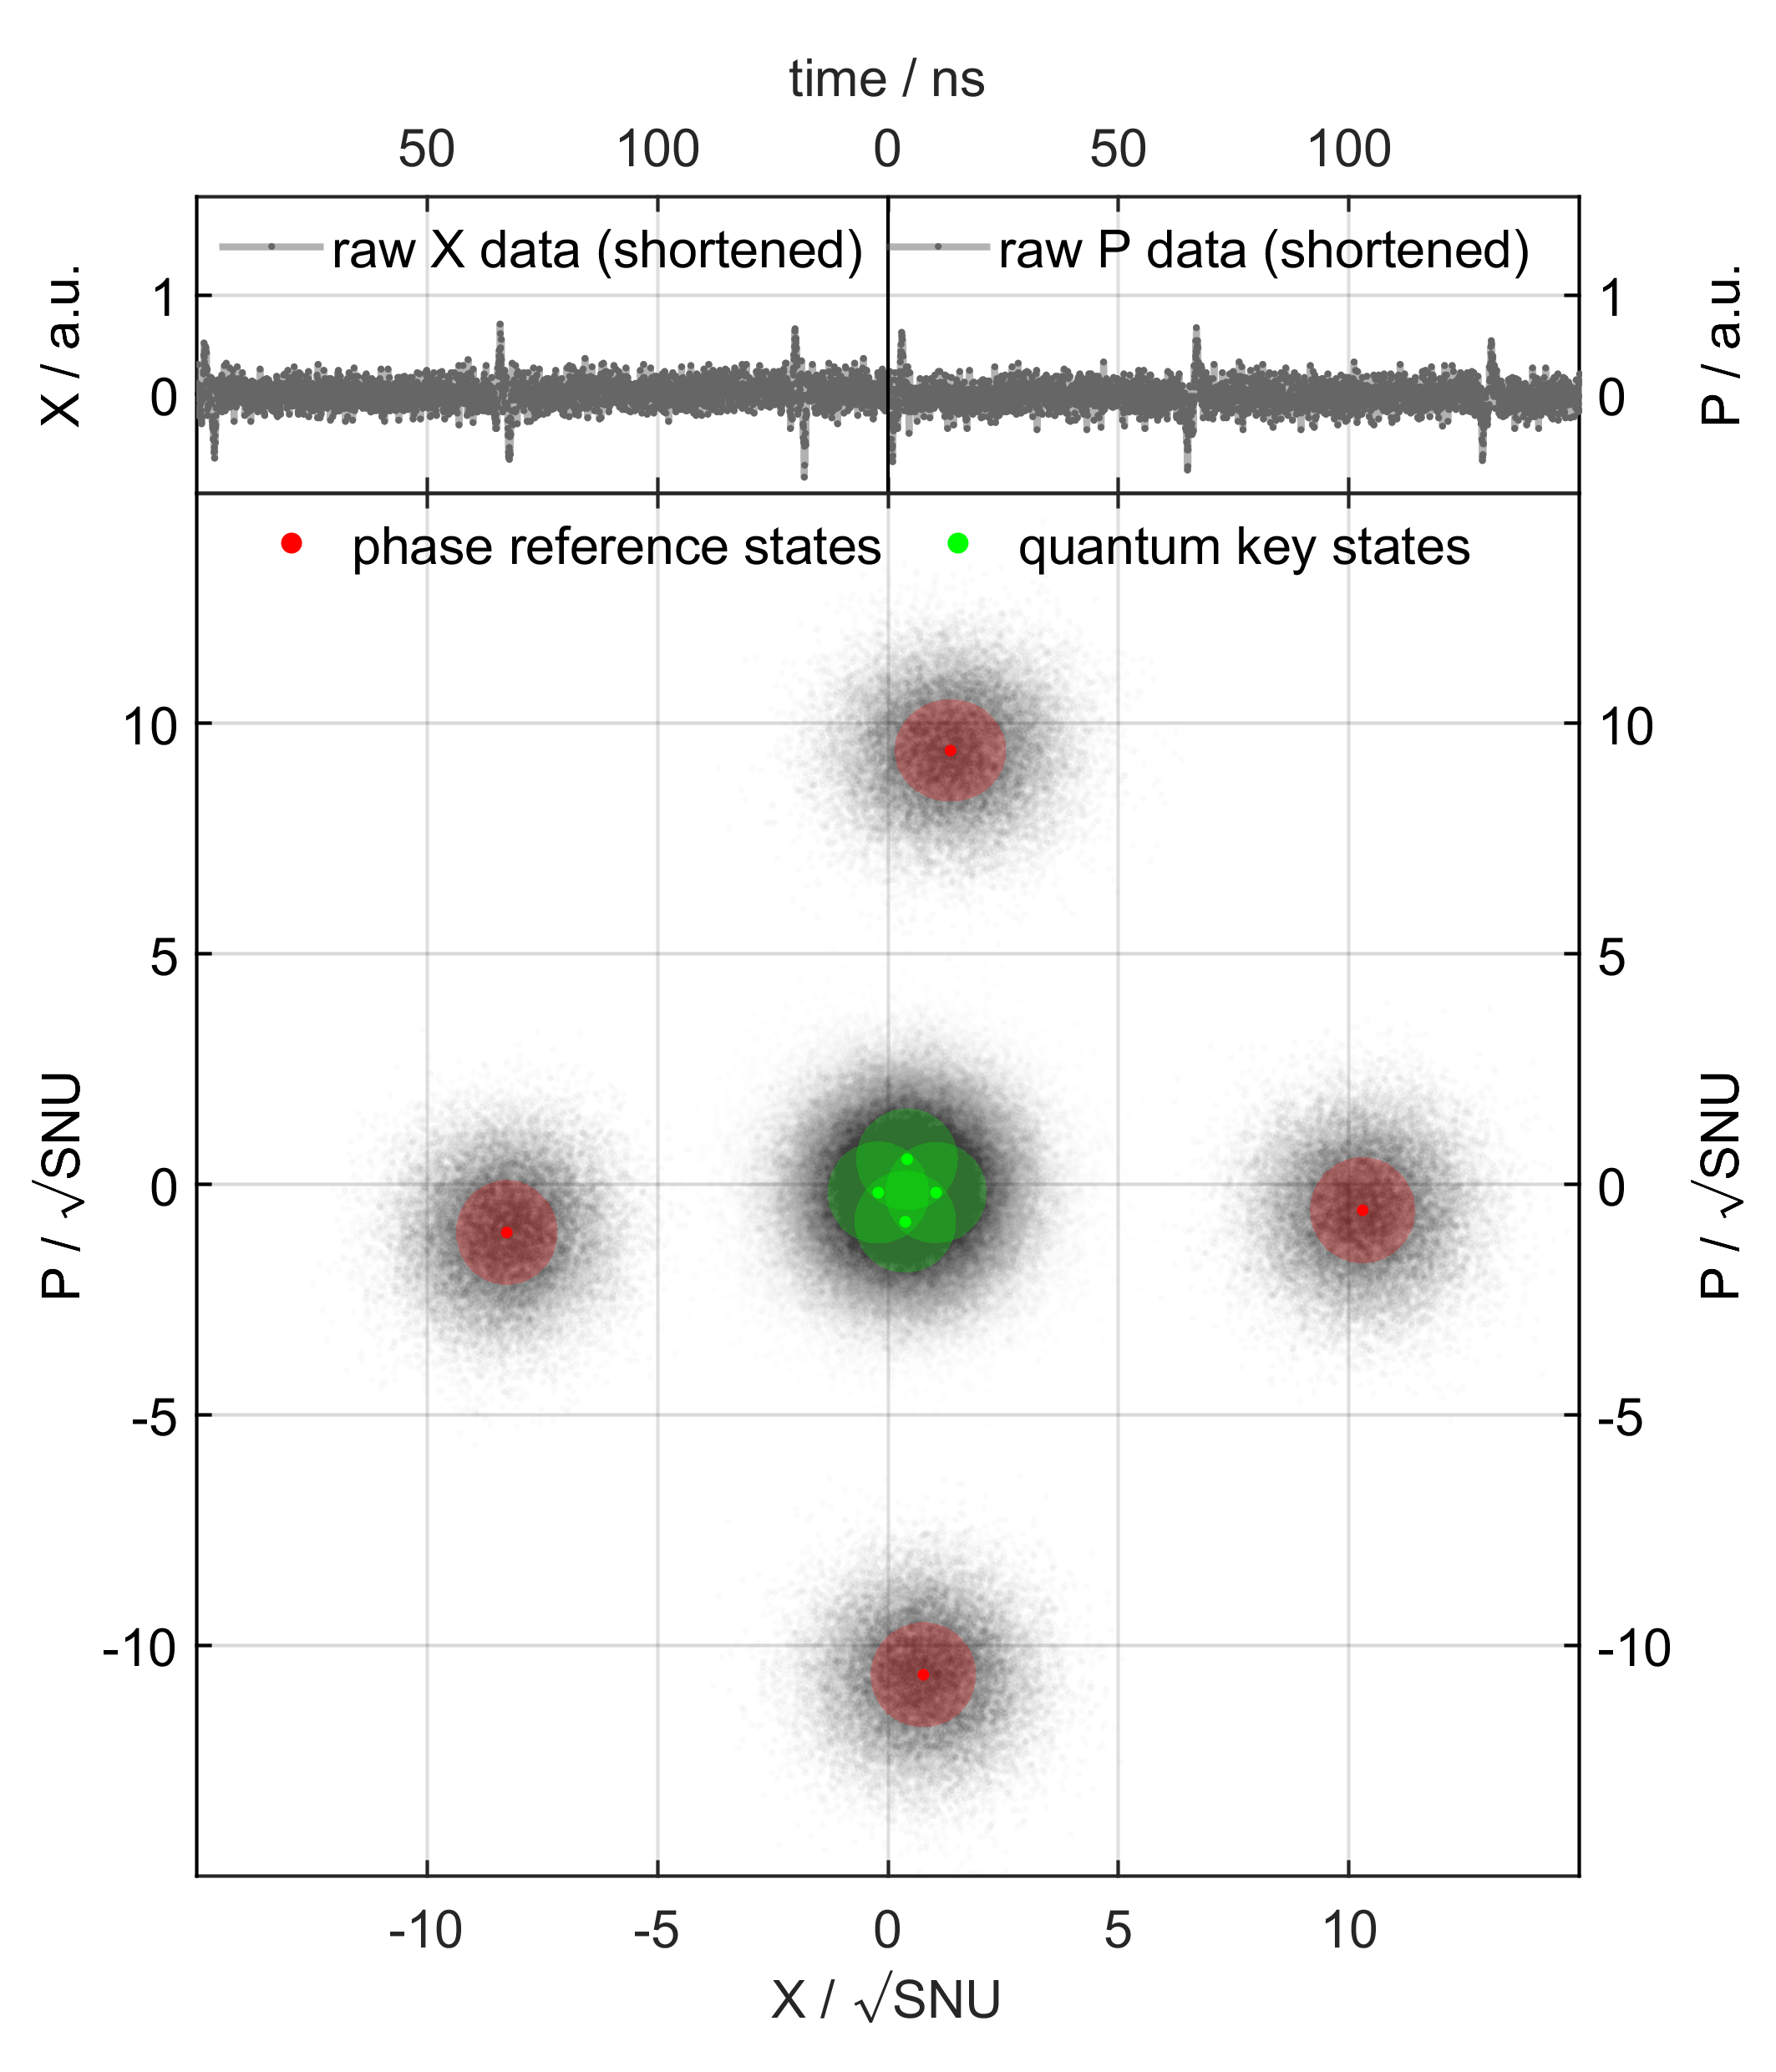
\includegraphics[draft=false, width=0.8\linewidth]{aqc/QDS_dataplots}
\caption{\label{fig:aqc_experimental_trace} Top: raw data trace. Bottom: data after DSP. Red: heterodyne outcomes on bright phase-reference states, amplitude $\alpha^\prime$ which are sent at the start of each frame, and allow the phases of the remaining states to be reconstructed. Green: heterodyne measurement outcomes on signal states amplitude $\alpha < \alpha^\prime$. The cryptographic tasks are performed with signal (green) data points only. \emph{Picture credit: Stefan Richter in Ref.~\cite{Richter2020}}
%Top: Raw quadrature data produced by the experiment detailed in Sec.~\ref{sec:aqc_experiment}. The raw data undergoes a proprietary digital signal processing (DSP), and produces the phase-space constellation displayed in the bottom diagram. Each black point is a measurement outcome. Shaded circles represent the means and variances of the received outcomes. Red: phase reference states. Green: signal states. \emph{Picture credit; Stefan Richter in Ref.~\cite{Richter2020}
}
\end{figure}

\clearpage
\section{Data analysis}
In this section we will analyse the data which was obtained in the experiment detailed in the previous section. Our starting point is the signal data points\footnote{Green in Fig.~\ref{fig:aqc_experimental_trace}} which we received from MPL. In Sec.~\ref{sec:aqc_protocol_modifications} we will demonstrate how the cryptographic protocols detailed above may be altered to more closely match the realistic data which includes experimental imperfections. %The ideal figures of merit obtained previously should be interpreted as upper bounds to protocol performance.
In Sec.~\ref{eqn:aqc_received_data} we will closely examine the data which we have received from MPL and which forms the basis for our demonstration of two quantum agile systems. We will demonstrate how it may be used to estimate protocol performance and figures of merit\footnote{Of which the ideal figures of merit obtained in previous chapters are an upper bound}, and then discuss how how the experiment lends itself to an agile interpretetation.

%\MT{Do some quick analysis of the data here, since I will want to refer to it in the Protocol modifications section.}

\subsection{Protocol modifications}\label{sec:aqc_protocol_modifications}
Throughout this Thesis it has been assumed that an ideal QPSK alphabet has been distributed, with states chosen uniformly and at random. This has allowed us to make several simplifying assumptions. For example in protocol QDS-$f$, these assumptions allowed us to simplify Eq.~\ref{eqn:aposteriori_entropy} as follows
\begin{equation}
\sum_{e_k} \text{P}\left(e_k\right) S\left(\rho_{\left. B \given e_k\right.}\right) \rightarrow S\left(\rho_{\left. B \given e_1\right.}\right).
\end{equation}

\noindent Similarly, in QSS-$b$ we repeatedly used the fact that each QPSK state was equally likely, in order to write Eq.~\ref{eqn:qss_deriv_3}, for example, as
\begin{equation}
\text{P}\left(b, c\right) = \frac{1}{16}.
\end{equation}

\noindent Realistically the states are not sent with identical sending probabilities, nor are they sent with identical amplitudes. The actual sending amplitudes for each experimental run are displayed in Tab.~\ref{table:aqc_data_parameters}. Non-uniform sending probabilities may also be directly measured from a disclosed subset of data. These imperfections must be taken into account in our bounds for key rate and signature length, which we now do.

\subsubsection{QDS-$b$}
In QDS-$b$ the key parameter to calculate is $g_{\text{sec}} = \pe - \perr$, which is related to the signature length figure of merit via Eq.~\ref{eqn:aqc_qdsb_efail}. Bob's mismatch probability $\pe$ is made more realistic by changing several steps in the derivation of Holevo information $\chi$. 

For example, under attack BS$0$ we update Bob's \emph{a priori} state, c.f. Eq.~\ref{eqn:qdsb_apriori_state} to be
\begin{equation}
\rho_B = \sum_{\alpha_k} \text{P}\left(\alpha_k\right) \dyad{\sqrt{1-T} \alpha_k}
\end{equation}
where the amplitudes $\alpha_k$ and sending probabilities $\text{P}\left(\alpha_k\right)$ are directly derived from the received data. Bob's \emph{a posteriori} states 

\begin{equation}
\rho_B^k = \dyad{\sqrt{1-T}\alpha_k},
\end{equation} 
and \emph{a posteriori} entropy
\begin{equation}
\sum_{\alpha_k}\text{P}\left(\alpha_k\right) S\left(\rho_B^k\right),
\end{equation}
now also depend on the measured data. For attacks BS$1$ and EC, they must be calculated without the simplifications afforded by ideal sending probabilities and equal $\left|\alpha_k\right|$'s. For attack BS$0$ Bob's \emph{a posteriori} entropy vanishes identically because his state is pure.

The honest mismatch probability $\perr$ may be measured directly from the data by observing the probability that a state is eliminated. We demonstrate this in Sec.~\ref{sec:aqc_performance}.


\subsubsection{QSS-$b$}
We will demonstrate the necessary alterations which should be made to mutual information I and Holevo information $\chi$ in protocol QSS-$b$.

\paragraph{Mutual Information I, Eq.~\ref{eqn:qss_deriv_1}}
The joint Shannon entropy of Bob and Charlie's variables is given by
\begin{equation}
\text{H}\left(X_B, X_C\right) = - \sum_{X_B=b, X_C=c} \text{P}\left(b, c\right) \log \text{P}\left(b, c\right)
\end{equation}
where $X_B, X_C$ denote the states from QPSK which Bob and Charlie sent, and $\text{P}\left(b, c\right)$ their sending probabilities. We have observed that
\begin{equation}
\text{P}\left(b, c\right) = \text{P}\left(b\right) \times \text{P}\left(c\right)
\end{equation}
and when variations in the sending probabilities are considered this is no longer equal to $1/16$. 

Secondly, the probability $\text{P}\left(X_A=a \given X_B=b, X_C=c\right)$, Eq.~\ref{eqn:qss_prob2}, should be updated to match the actual amplitudes of the sent coherent states.

\paragraph{Holevo information $\chi$}
The initial states Eq.~\ref{eqn:qss_initial_states} should be updated to
\begin{equation}
\rho_B = \sum_{k=0}^3 \text{P}\left(\beta_k\right) \dyad{\beta_k}_B \qq{and} \rho_C = \sum_{k^\prime=0}^3 \text{P}\left(\gamma_{k^\prime}\right) \dyad{\gamma_{k^\prime}}_C
\end{equation}
and therefore Eq.~\ref{eqn:qss_deriv_8} becomes
\begin{align}
&\rho_{\left.\mathbb{E} \given X_A, A_B\right.} = \frac{1}{\pi^2}\sum_{k, k^\prime=0}^3 \text{P}\left(b, c\right) \text{P}_B\left(A_B \given \beta_k, T_B\right) \text{P}C\left(\frac{X_A - g A_B}{h} \given \gamma_{k^\prime}, T_C\right) \notag \\
&\dyad{\sqrt{1-T_B}\beta_k}_{\mathbb{E}_B} \otimes \dyad{\sqrt{1-T_C} \gamma_{k^\prime}}_{\mathbb{E}_C}
\end{align}
from which Holevo information $\chi$ is calculated.

\subsubsection{QDS-$f$}
Protocol QDS-$f$ requires us to recalculate $g_{\text{sec}} = \pe - \perr$ with these experimental imperfections. Probability $\perr$ may be estimated directly from data and is equivalent to the analysis performed above for QDS-$b$.

Probability $\pe$ requires us to reconsider certain steps in the calculation of Holevo information $\chi$. We consider attack BS$0$, and other attacks follow suit. After the channel, the state held by Charlie and dishonest Bob is, c.f. Eq.~\ref{eqn:qds_after_channel},

\begin{equation}
\sum_{\alpha_k} \text{P}\left(\alpha_k\right)  \left[ \dyad{\sqrt{T}\alpha_k}_C \otimes \dyad{\sqrt{1-T}\alpha_k}_B\right],
\end{equation}
and so Bob's conditional state becomes, c.f. Eq.~\ref{eqn:qds_bob_conditional_state}
\begin{equation}
\rho_{\left.B \given c\right.} = \frac{1}{\text{P}\left(c\right)} \sum_{\alpha_k} \text{P}\left(\alpha_k\right) \text{P}\left(c \given \alpha_k, T\right) \times \dyad{\sqrt{1-T}\alpha_k}_B
\end{equation}
where $\text{P}\left(c \given \alpha_k, T\right)$ is Charlie's probability to measure $c$ and $\text{P}\left(c\right) = \sum_{\alpha_k}\text{P}\left(c \given \alpha_k, T\right)$ which is now no longer symmetric.

Each of Bob's states conditioned on an eliminated signature element $e_k$ now have different entropies and different probabilities $\text{P}\left(e_k\right)$ and so we must write the Holevo information out in full, c.f. Eq.~\ref{eqn:qds_deriv_holevo},

\begin{equation}
\chi = S\left(\sum_{e_k} \text{P}\left(e_k\right) \rho_{\left.B\given e_k\right.}\right) - \sum_{e_k} \text{P}\left(e_k\right) S\left(\rho_{\left.B\given e_k\right.}\right)
\end{equation}

\subsubsection{QKD-$f$}


%\MT{Do I want a graph of how this affects Eve's Holevo information, for example?}

Finally, we consider how the protocol QKD-$f$ may be updated to allow for non-uniform QPSK alphabets.

\paragraph{Mutual Information I, Eq.~\ref{eqn:qkdf_deriv_1}}

The Shannon entropy $\text{H}\left(X_A\right)$ of Alice's variable is easily modified with the new probability distribution $\text{P}\left(X_A\right)$, and is given by
\begin{equation}
\text{H}\left(X_A\right) = - \sum_{X_A=a} \text{P}\left(a\right) \log \text{P}\left(a\right)
\end{equation}
which is easily calculated using the measured $\text{P}\left(a\right)$. The conditional entropy $\text{H}\left(X_A \given X_B\right)$ is readily calculated following the discussion\footnote{See also the discussion for alterations to protocol QSS-$f$, which is analogous.} beneath Eq.~\ref{eqn:qkdf_deriv_2}.

\paragraph{Holevo information $\chi$}
Eve's conditional state after Bob's heterodyne measurement becomes, c.f. Eq.~\ref{eqn:qkdf_eve_conditional},
\begin{equation}\label{eqn:qkdf_eve_conditional_modified}
\rho_{\left. E \given b\right.} = \frac{1}{\text{P}\left(b\right)} \sum_{\alpha_k} \text{P}\left(\alpha_k\right) \text{P}\left(b \given \alpha_k, T\right) \times \dyad{\sqrt{1-T}\alpha_k}_E,
\end{equation}
with $\text{P}\left(b\right) = \sum_{\alpha_k} \text{P}\left(b \given \alpha_k, T\right)$ also changing and becoming asymmetric. 

Eve's \emph{a posteriori} and \emph{a priori} entropies are calculated identically to Eqs.~\ref{eqn:qkdf_aposteriori_entropy},~\ref{eqn:qkdf_apriori_entropy} using Eq.~\ref{eqn:qkdf_eve_conditional_modified} as a starting point.


%\clearpage
\subsection{Received data}\label{sec:aqc_received_data}
From our experimental collaborators at MPL we received four datasets output from the experiment detailed in Sec.~\ref{sec:aqc_experiment}. Figure~\ref{fig:aqc_dataplots_stefan} displays raw data before and after the action of the experimental collaborators' proprietary digital signal processing (DSP) algorithm. The data we have received is of the form of bottom figure of Fig.~\ref{fig:aqc_dataplots_stefan}, and we received only the signal data (green circles) once the phase-reference data (red circles) was removed. Each of the received datasets consisted of $1.54\times10^6$ elements of pairs of measured phase outcomes $\left(x_{\text{out}}, p_{\text{out}}\right)$, along with information about which element from the QPSK alphabet Alice sent. The received datasets have parameters detailed in Tab.~\ref{table:aqc_data_parameters}.

%\begin{figure}[htp]
%\centering
%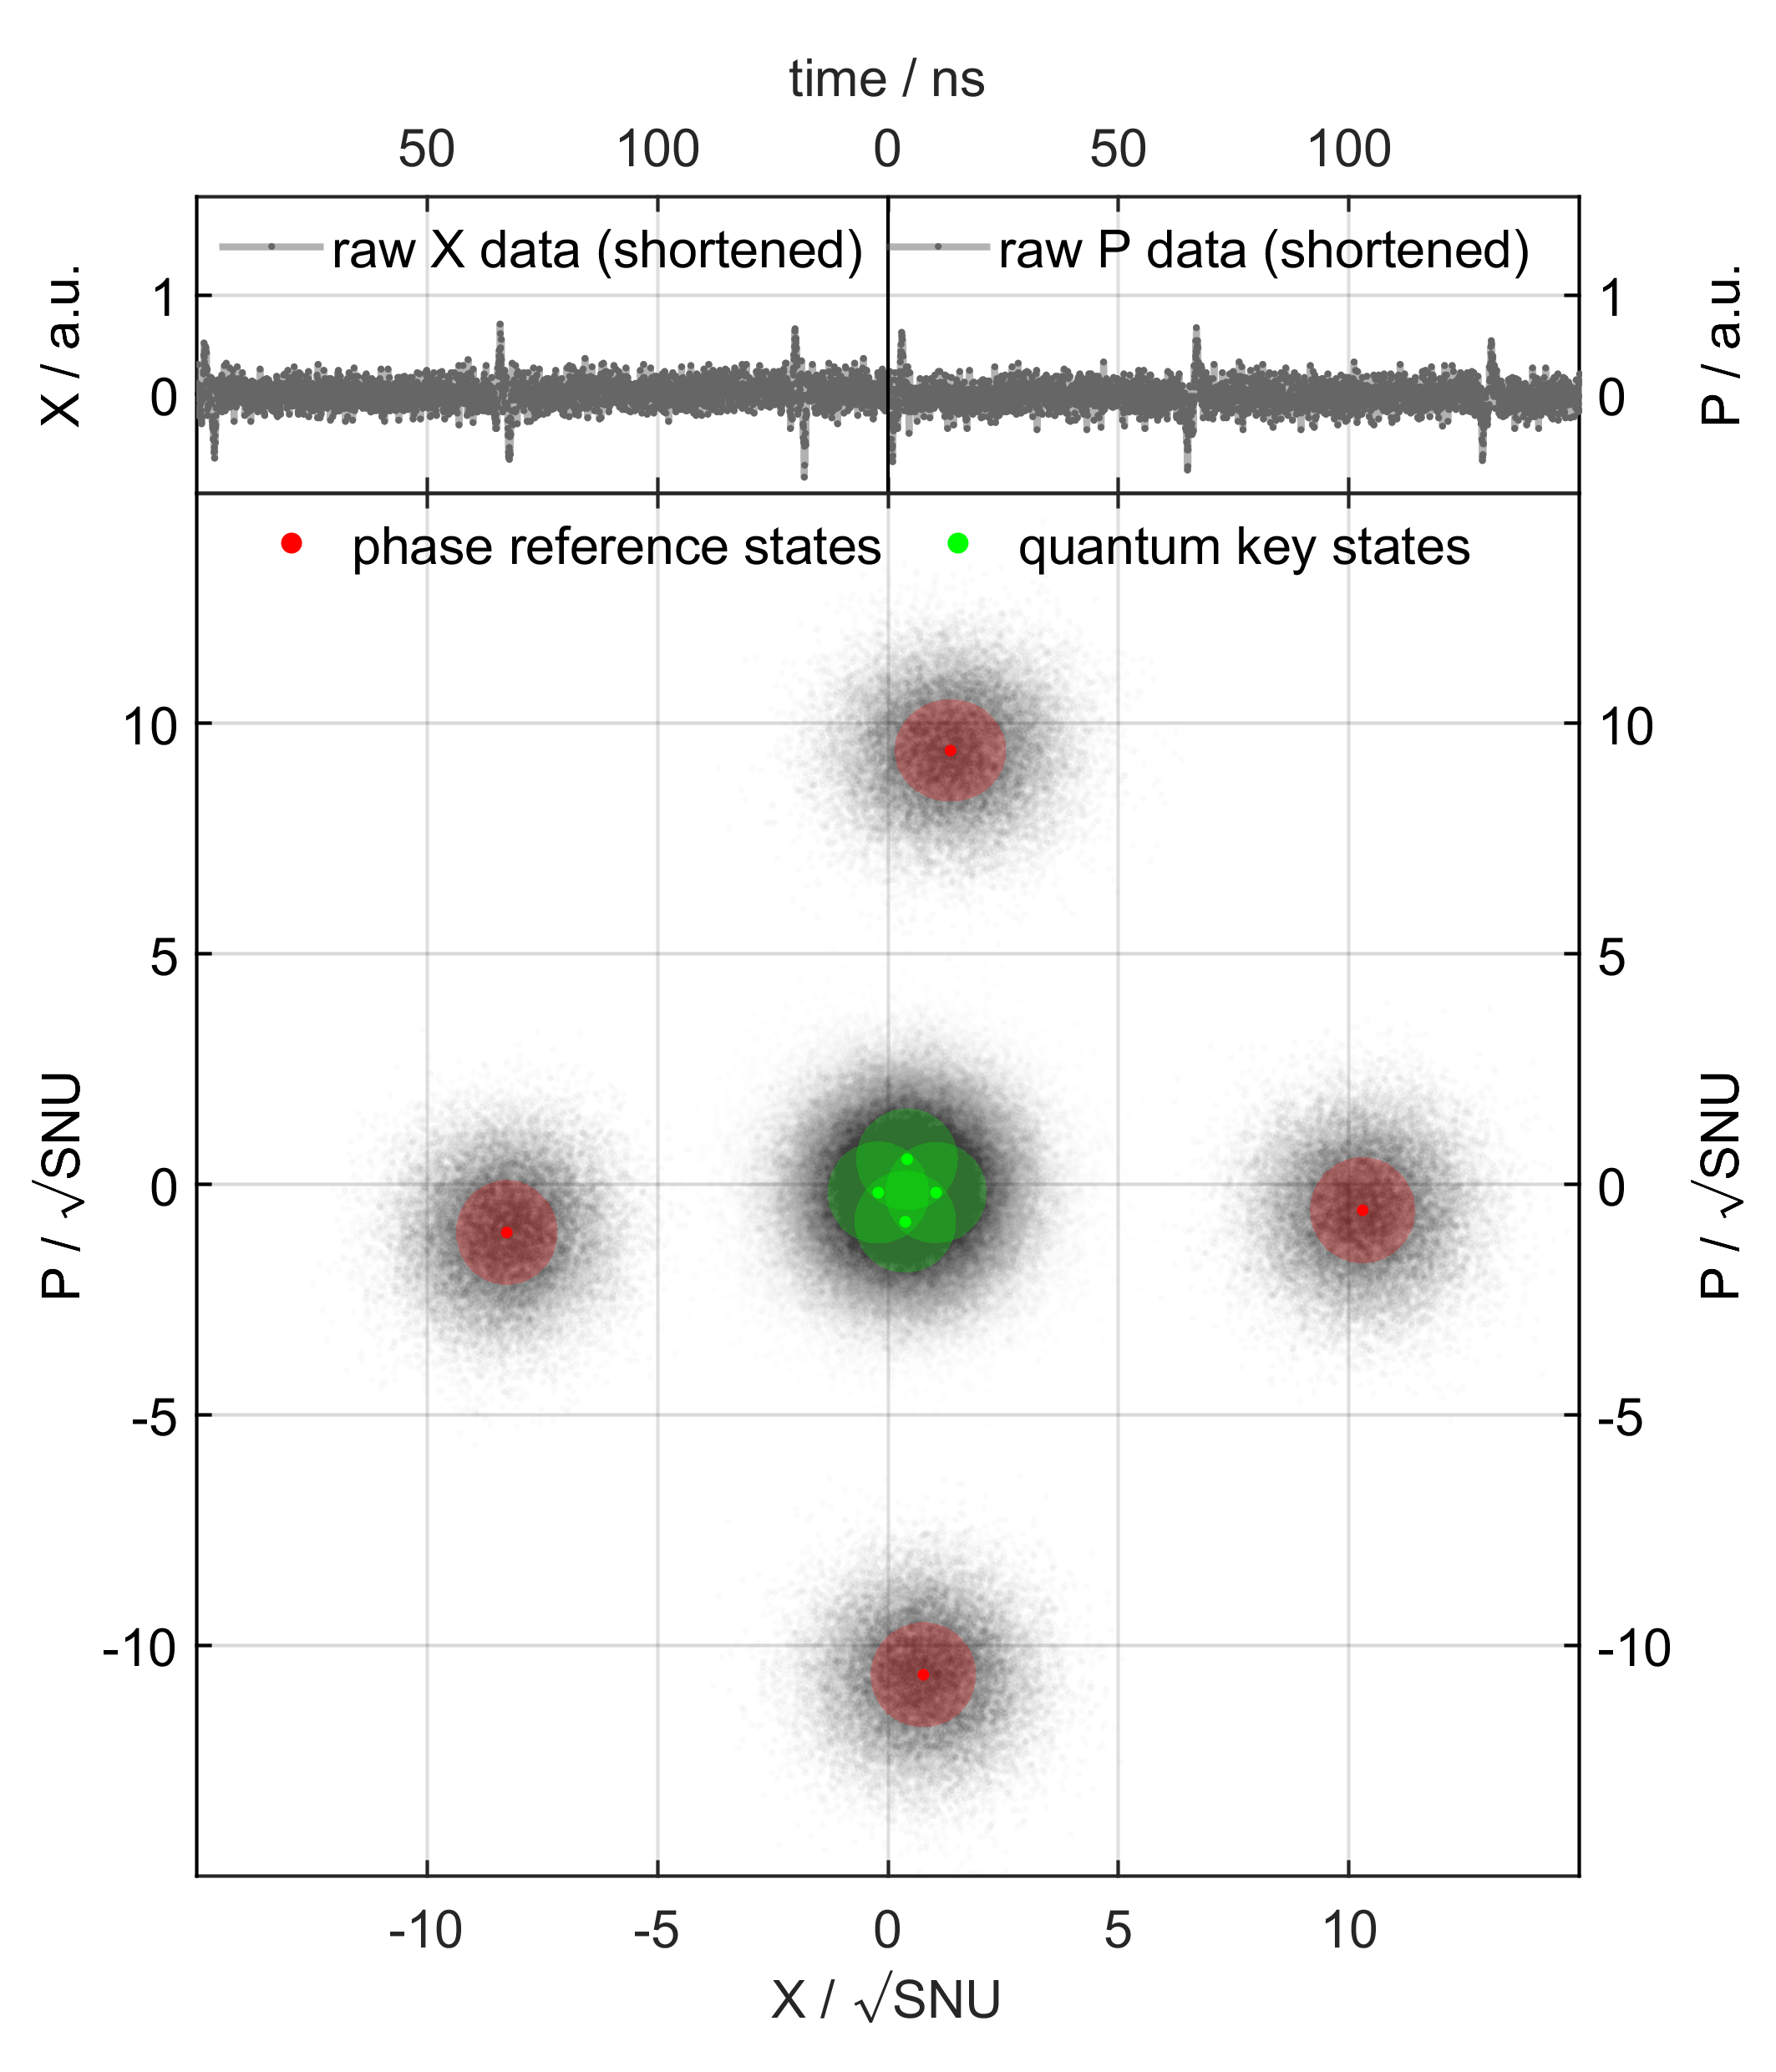
\includegraphics[width=0.6\linewidth, draft=false]{aqc/QDS_dataplots}
%\caption{\label{fig:aqc_dataplots_stefan} Top: Raw quadrature data produced by the experiment detailed in Sec.~\ref{sec:aqc_experiment}. The raw data undergoes a proprietary digital signal processing (DSP), and produces the phase-space constellation displayed in the bottom diagram. Each black point is a measurement outcome. Shaded circles represent the means and variances of the received outcomes. Red: phase reference states. Green: signal states. \emph{Picture credit; Stefan Richter in Ref.~\cite{Richter2020}}}
%\end{figure}

We calculate the parameters entering Tab.~\ref{table:aqc_data_parameters} directly from the received data sets. The amplitude $\alpha$ sent by Alice is calculated by a rescaling of phase measurement data, as follows. For data when a particular $\ket{\alpha}$ was sent, we calculate the means $\bar{x}_{\text{out}}$, $\bar{p}_{\text{out}}$ of measured output data. The mean coherent state amplitude which was received at Rx is then given by 
\begin{equation}
\alpha_{\text{Rx}} = \frac{\bar{x}_{\text{out}} + i \bar{p}_{\text{out}}}{\sqrt{2}}.
\end{equation}
From Tx to Rx, the distributed state has undergone two primary sources of loss: trusted loss and untrusted loss. Untrusted loss must be attributed to Eve, and is a combination of propagation losses in the fiber, and coupling losses into and out of the fiber. \MT{Check this. Have I received info from MPL at all ever?} We write this as a single number which corresponds to the loss of the channel (or channel transmission $T$), and is $-0.65$~dB for the $2$~km channel and $-4.75$~dB for the $20$~km channel. These values were given to us by our experimental collaborators and were measured using their proprietary methods. The trusted loss occurs in the detector Rx and an eavesdropper is assumed to not have access to this. The quoted value is $\approx 50\%$ loss due to Rx.

The amplitude sent by Tx may then be calculated as
\begin{equation}
\alpha_{\text{Tx}} = \frac{\alpha_{\text{Rx}}}{\sqrt{0.5} \sqrt{T}}.
\end{equation}
This scaling procedure was done for each run and each distributed QPSK state, and the re-scaled values are displayed in Tab.~\ref{table:aqc_data_parameters}.

The excess noises corresponding to measurements in each quadrature $\xi_x$, $\xi_p$ are calculated separately, and the value of excess noise which we use to estimate the power of the eavesdropper is $\xi = \max \left\{\xi_x, \xi_p\right\}$. Maximizing $\xi$ in this way gives the eavesdropper additional power, since it assumes that they have used a state with a higher degree of entanglement. We might reasonably expect that affording Eve this power should loosen the bounds which we calculate in this chapter, and tighter bounds with an analysis which includes this asymmetry in noise profiles are left for future work.

The variance in measurement outcome in each $x$ and $p$ for each distributed state was measured, and the final excess noise is given by
\begin{equation}
\xi_{x} = \text{Var}\left(x\right) - \frac{1}{2} - \text{Var}\left(x\right)_{\text{trusted}},
\end{equation} %Check whether it should be 1 or 1/2.
and similarly for $p$. The contribution $\text{Var}\left(x\right)_{\text{trusted}}$ represents system detector noise which is assumed to be outside of Eve's control, and which was fully characterised by our experimental collaborators. The final excess noise values are then averaged over each distributed QPSK state, and then maximized over $x, p$. These final values $\xi$ are displayed in Tab.~\ref{table:aqc_data_parameters}. The excess noise values were quoted to us by experimental collaborators.



\begin{table*}%[hb!p]
	\captionsetup{width=0.8\linewidth}
	\centering \ra{1.75}
	\begin{tabular*}{\textwidth}{@{\extracolsep{\stretch{1}}}  cc c ccccc c c }
	%\toprule
	% primary header
	\multicolumn{2}{c}{\textbf{Experiment}} &&
	\multicolumn{5}{c}{\textbf{QPSK amplitudes} $[\sqrt{\text{snu}}\,]$} &&
	\multicolumn{1}{l}{\textbf{Excess noise} $[\si{\%}]$} \\
%	\colrule
	\hline
	%\cline{1-4}\cline{6-7} \cline{9-10}\cline{12-12}
	% secondary header
%	\text{Run} & \head{$d\,[\si{km}]$} & \head{$\bar{\alpha}\,[\sqrt{\text{snu}}\,]$} & \head{$\xi\,[\si{\%}]$} &&
%	\head{$L\,[\si{bits^{-1}}]$} & \head{$t\,[\si{ms}]$} &&
%	\head{$L\,[\si{bits^{-1}}]$} & \head{$t\,[\si{ms}]$} &&
%	\head{$2 \kappa$}  && 
%	\head{$\kappa$}
%	\\
	\head{Run} & \head{Fiber $[\si{km}]$} &&
	\head{$\alpha$} & \head{$i \alpha$} & \head{$- \alpha$} & \head{$- i \alpha$} & \head{$\bar{\alpha}$} &&
	\head{$\max\left\{\xi_x, \xi_p \right\}$}
	\\
%	\colrule
\hline
	% table body
	1 & 2 && 0.615 & 0.676 & 0.620 & 0.620 & 0.64 && 2.7\\
	2 & 20 && 0.624 & 0.754 & 0.629 & 0.717 & 0.67 && 1.9\\
	3 & 20 && 0.493 & 0.626 & 0.499 & 0.606 & 0.55 && 2.1\\
	4 & 20 && 0.578 & 0.716 & 0.579 & 0.688 & 0.64 && 1.7\\
	%\botrule
	\end{tabular*}
	\caption{\label{table:aqc_data_parameters} Parameters of received datasets. Each of the four experimental runs had slightly asymmetric amplitudes for each of the QPSK alphabet states $\alpha$, $i \alpha$, $- \alpha$, $- i \alpha$. The mean amplitude for each run is $\bar{\alpha}$. Each of the states was sent with probability close to $1/4$. Excess noise differs between $x$ and $p$ quadratures, and for our analysis the largest of these was chosen, i.e. $\xi = \max\left\{\xi_x, \xi_p\right\}$. The loss level corresponding to the $2$~km channel is $-0.65$~dB, and the loss level corresponding to $20$~km channel is $-4.75$~dB. This includes the channel and additional losses due to coupling inefficiencies, but does not include trusted detector loss of $50\%$. }
\end{table*}



To illustrate our received data, we plot the first $10,000$ elements of raw data for run~$1$ in Fig.~\ref{fig:aqc_scatter}. In (a) we display data corresponding to the input state $\ket{\alpha}$ with $\alpha=0.615$, and in (b) we display data corresponding to the entire QPSK alphabet, which is highly non-orthogonal.



\begin{figure}[htp]
\captionsetup{width=0.8\linewidth}
\centering
	\begin{subfigure}{0.49\linewidth}
	\centering
	\includegraphics[width=\linewidth, draft=false]{aqc/scatter_1}
	\caption{}
	\end{subfigure}
	\begin{subfigure}{0.49\linewidth}
	\centering
	\includegraphics[width=\linewidth, draft=false]{aqc/scatter_2}
	\end{subfigure}
\caption{\label{fig:aqc_scatter} Datasets received from experimental collaborators, corresponding to $x_{\text{out}}$ and $p_{\text{out}}$ phase measurement outcomes when (a) state $\ket{\alpha}$ was sent, run~$1$ and (b) states $\ket{\alpha}$, $\ket{i \alpha}$, $\ket{- \alpha}$, $\ket{- i \alpha}$ were sent, run~$1$. We plot only the first $10,000$ points, for illustrative convenience. (b) At the amplitudes chosen, our QPSK alphabet is overlapping and highly non-orthogonal.}
\end{figure}

In Fig.~\ref{fig:aqc_elimsig} we demonstrate for protocols QDS-$f$ and QDS-$b$ how $\perr$ may be calculated on a particular dataset. Having isolated the elements for which a particular alphabet state was sent, the data is partitioned into groups which will induce a mismatch. In this case, $\ket{\alpha}$ was sent and so data with $x_{\text{received}} \ge 0$ will not induce a mismatch, while data with $x_{\text{received}}<0$ will. The mismatch probability $\perr$ is then calculated as
\begin{equation}\label{eqn:aqc_data_perr}
\perr = \frac{\text{Number of data points which cause a mismatch}}{\text{Total number of data points}},
\end{equation}
where the numerator is calculated including all four of the distributed QPSK states, with their respective mismatch criteria.

\begin{figure}[htp]
\captionsetup{width=0.8\linewidth}
\centering
\includegraphics[width=0.6\linewidth, draft=false]{aqc/eliminated_signature_data}
\caption{\label{fig:aqc_elimsig} Illustration of received data points, coloured by whether they induce a mismatch in protocols QDS-$f$ and QDS-$b$. State $\ket{\alpha}$ was sent, and data is taken from run~$1$. Blue: data points will not cause $\ket{\alpha}$ to be eliminated, and so do not cause a mismatch. Red: data points will cause $\ket{\alpha}$ to be eliminated, and so a mismatch occurs. \MT{TODO: Change axis labels for consisteny. Q: how many points are here?}}
\end{figure}

In protocols QDS-$f$ and QDS-$b$ we also discussed the possibility to postselect on measurement outcomes, by ignoring datapoints which fall within $\rps$. As was discussed in their respective sections we take $\rps\left(\Delta_r\right)$, and display examples of postselected data sets in Fig.~\ref{fig:aqc_ps}. Data corresponding to distributed $\ket{\alpha}$ are displayed in Fig.~\ref{fig:aqc_ps}a, while data for all elements of QPSK are displayed in Fig.~\ref{fig:aqc_ps}b. For illustrative convenience we display only the first $10,000$ elements. We may calculate $\perr$ in an identical way to that discussed above, simply starting from the postselected data in order to reduce $\perr$ and increase the advantage gained by an honest player.

\begin{figure}[htp]
\captionsetup{width=0.8\linewidth}
\centering
	\begin{subfigure}{0.49\linewidth}
	\centering
	\includegraphics[width=\linewidth, draft=false]{aqc/scatter_PS_1}
	\caption{}
	\end{subfigure}
	\begin{subfigure}{0.49\linewidth}
	\centering
	\includegraphics[width=\linewidth, draft=false]{aqc/scatter_PS_2}
	\caption{}
	\end{subfigure}
\caption{\label{fig:aqc_ps} Postselection technique with region $\rps\left(\Delta_r=1.0\right)$ applied to the datasets from Fig.~\ref{fig:aqc_scatter}.}
\end{figure}


\clearpage
\subsection{Protocol performance}\label{sec:aqc_performance}
The experiment detailed in Sec.~\ref{sec:aqc_experiment} was  performed and we have received four datasets from our experimental collaborators. The key parameters for these datasets are described in Tab.~\ref{table:aqc_data_parameters} and form the basis for an analysis of performance of each of our cryptosystems.

%\iffalse
\begin{table*}%[hb!p]
	\captionsetup{width=0.8\linewidth}
	\centering \ra{1.75}
	\begin{tabular*}{\textwidth}{@{\extracolsep{\stretch{1}}} c  cccc c rr c rr c r cc}
	%\toprule
	% primary header
%	\multicolumn{4}{c}{\textbf{Experiment}} &&
	\multicolumn{1}{c}{\textbf{}} &&
	\multicolumn{2}{c}{\textbf{QDS\,-\,$b$}} &&
	\multicolumn{2}{c}{\textbf{QDS\,-\,$f$}} &&
	\multicolumn{1}{c}{\textbf{QSS\,-\,$b$}} && 
	\multicolumn{1}{c}{\textbf{QKD\,-\,$f$}} \\
%	\colrule
	\hline
	%\cline{1-4}\cline{6-7} \cline{9-10}\cline{12-12}
	% secondary header
%	\text{Run} & \head{$d\,[\si{km}]$} & \head{$\bar{\alpha}\,[\sqrt{\text{snu}}\,]$} & \head{$\xi\,[\si{\%}]$} &&
	\head{Run} &&
	\head{$L\,[\si{bits^{-1}}]$} & \head{$t\,[\si{ms}]$} &&
	\head{$L\,[\si{bits^{-1}}]$} & \head{$t\,[\si{ms}]$} &&
	\head{$2 \kappa$}  && 
	\head{$\kappa$}
	\\
%	\colrule
\hline
	% table body
	 1 && $\enot{5.70}{6}$ & $5.7$ && $\enot{4.79}{4}$ & $0.048$ && 0.3726 && 0.3479\\
2 && - &        - && $\enot{2.26}{9}$ &  $2260$ && 0.1058 && 0.1024\\
3 && - &        - && $\enot{1.37}{8}$ &    $137$ && 0.0858 && 0.0840 \\
4 && - &        - && $\enot{2.08}{8}$ &    $208$ && 0.1004 && 0.0976\\
	%\botrule
	\end{tabular*}
	\caption{\label{tab:lengths} Protocol figures of merit for the experimental runs. QDS signature lengths (L) and signing times (t) required to sign a $1$-bit message for security level of $\varepsilon = 0.001\%$. The QSS and QKD key rates correspond to the maximum estimated number of bits of secure key which may be generated per use of the quantum channel. In QSS-$b$, one channel use corresponds to distribution of \emph{two} quantum states, one from Bob and one from Charlie, and so we display $2 \kappa$ for fair comparison with QKD. \MT{Make sure that security level $\varepsilon$ is defined.}}
\end{table*}
%\fi

\subsubsection{First agile system \systemB}
In the first agile system, \systemB, the sender module Tx is understood to play the role of either Bob or Charlie, while Rx plays the role of Alice. Signature lengths under QDS-$b$ are calculated using the data parameters from Tab.~\ref{table:aqc_data_parameters} with the postselection region\footnote{$\rps = \mathcal{R}\left(\Delta_r\right)$} $\rps$ optimized. In the ideal case, honest mismatch probability $\perr$ is calculated using Eq.~\ref{eqn:perr} under the model described there (or including excess noise, Appendix~\ref{appendix:noisy_channel}). We additionally include a detector efficiency of $50\%$ which a dishonest player cannot exploit. 

For QDS-$b$ we allow dishonest Bob to perform the entangling cloner attack, and we estimate $\pe$ using the models in Sec.~\ref{sec:qds_attack_analysis},~\ref{sec:aqc_systemb} once $\alpha$ and the worst-case excess noise $\xi$ have been estimated from data. These ideal signature lengths for QDS-$b$ are displayed in Fig.~\ref{fig:aqc_qdsb}. The point at which run~$1$ (red) intersects the vertical gridline ($2$~km fiber length) corresponds to a point at which we have data. Other points in Fig.~\ref{fig:aqc_qdsb} are calculated by varying $T$ in our model.

We see that over metropolitan distances of up to several kilometers, which are favourable to the CV platform, the protocol QDS-$b$ obtains modest signature lengths $\mathcal{O}\left(10^6\right)$. At these short distances however the excess noise $\xi$ has strong impact on the required signature lengths.

\begin{figure}[htp]
\captionsetup{width=0.8\linewidth}
\centering
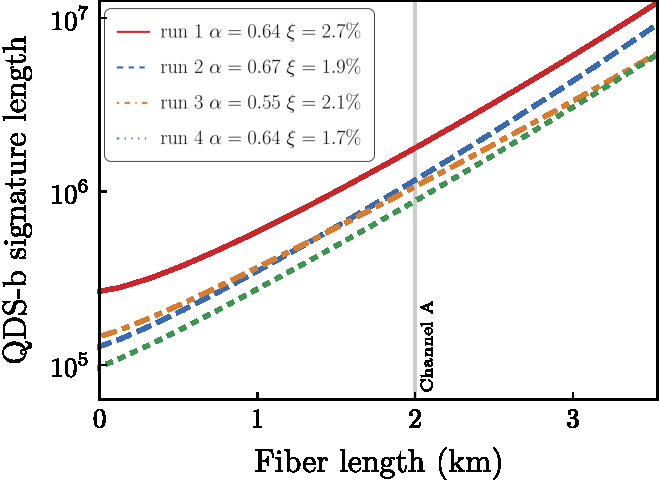
\includegraphics[draft=false, width=0.8\linewidth]{aqc/qdsb}
\caption{\label{fig:aqc_qdsb} Signature lengths required to sign a single bit in protocol QDS-$b$, under entangling-cloner attack. The signature lengths at a distance of $2$~km remain modest both in the ideal (above) and experimental (Tab.~\ref{table:lengths}) realizations. %The system is robust to choice of $\alpha$. 
Solid (red), dashed (blue), dot-dashed (orange) and dotted (green) lines correspond to performance deduced by parameters from experimental runs $1$, $2$, $3$ and $4$, respectively. The vertical grid line depicts the loss level over experimental channel $A$ ($0.65$~dB loss).}
\end{figure} %Make sure that channel A is described somewhere.

More realistic signature lengths may be calculated by taking into account in the estimate of $\pe$ the actual amplitudes and sending probabilities which Tx sent (Sec.~\ref{sec:aqc_protocol_modifications}), rather than their average, and additionally by measuring $\perr$ directly from the output of Rx. The $\perr$ calculated in this way automatically takes into account all sources of trusted detector loss and noise which will increase $\perr$. The actual measured $L$ will be larger than those displayed in Fig.~\ref{fig:aqc_qdsb}. 

For example, for experimental run~$1$ over the $2$~km channel (Channel A), a signature length of $5.7 \times 10^6$ is required to sign a single bit, Tab.~\ref{tab:lengths}. However, even at $20$~km protocol QDS-$b$ could still be made secure by choosing a postselection region with $\Delta_r \ggg 1$, but for loss levels larger than $\sim 2$~dB the required signature length becomes impractically large.

For our secret sharing protocol QSS-$b$, Fig.~\ref{fig:aqc_qssb}, the Holevo information is calculated by estimating channel transmission $T$ and excess noise $\xi$ from the data and assuming that the dishonest players perform beamsplitter attack BS$2$ (Sec.~\ref{sec:qds_attack_analysis}). The mutual information is obtained by calculating the probability $p\left(x \given \alpha_k\right)$ of measuring $x$ at the output when coherent state $\alpha_k$ was sent.% noting again that the realistic non-identical amplitudes and sending probabilities of the implemented QPSK alphabet may be readily included.

Maximum QSS key rates, calculated from measured experimental parameters Tab.~\ref{table:aqc_data_parameters} with modifications from Sec.~\ref{sec:aqc_protocol_modifications}, are displayed in Tab.~\ref{tab:lengths}. We see that twice the key rate, $2 \kappa$ is greater than the comparable key rate $\kappa$ for QKD-$f$ (remembering that one channel use is defined differently between QKD and QSS). In other words, QSS-$b$ outperforms pairwise QKD by consuming fewer quantum resources to obtain an equivalent key rate. We have observed therefore that a ``direct'' QSS can outperform the classical unconditionally secure secret sharing mediated by QKD. This is thus another case where our agile framework is preferable to the QKD-assisted crypto-agility.

\begin{figure}[htp]
\captionsetup{width=0.8\linewidth}
\centering
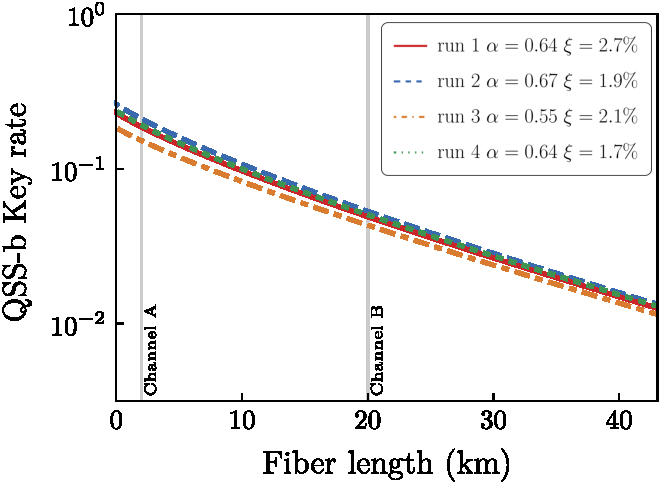
\includegraphics[draft=false, width=0.8\linewidth]{aqc/qssb}
\caption{\label{fig:aqc_qssb} Maximum attainable key rates for protocol QSS-$b$. Dishonest Eve performs attack BS$2$, and either Bob or Charlie are also dishonest. The key rate is robust to variations in $\alpha$, and remains large even for our $20$~km channel. Solid (red), dashed (blue), dot-dashed (orange) and dotted (green) lines correspond to the ideal performance deduced by parameters from experimental runs $1$, $2$, $3$ and $4$, respectively. Vertical grid lines depict loss levels over experimental channels $A$ and $B$, corresponding to fiber lengths $2$~km ($0.65$~dB loss) and $20$~km ($4.75$~dB loss)}
\end{figure}

\subsubsection{Second agile system \systemF}
For the second agile system, \systemF, Tx plays the role of Alice while Rx plays either Bob or Charlie. The performance under protocol QDS-$f$ is displayed in Fig.~\ref{fig:aqc_qdsf} under attack BS$2$. The excess noise and detector efficiency from the experiment are included, and $\pe$ and $\perr$ are calculated using analogous methods to QDS-$b$, above. We see than in the ideal analysis of Fig~\ref{fig:aqc_qdsf} (using models from Ch.~\ref{chapter:qds}) the protocol QDS-$f$ allows for very small signature lengths $\mathcal{O}\left(10^4\right)$ at $2$~km, while at $20$~km the predicted lengths are still very modest at $\mathcal{O}\left(10^6\right)$.

\begin{figure}[htp]
\captionsetup{width=0.8\linewidth}
\centering
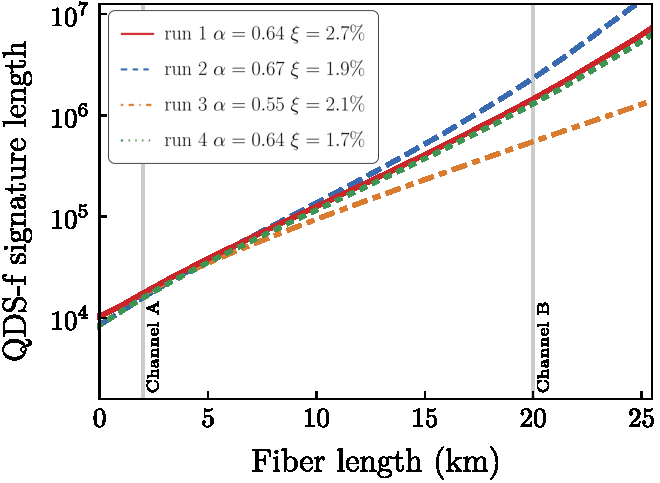
\includegraphics[width=0.8\linewidth, draft=false]{aqc/qdsf}
\caption{\label{fig:aqc_qdsf} Signature lengths required to sign a single bit in protocol QDS-$b$, under attack BS$2$. The signature lengths at $20$~km (Channel B) remain feasible under both ideal (above) and experimental (Tab.~\ref{tab:lengths} realizations. At $2$~km (Channel A) the protocol requires small signature lengths and is thus the fastest QDS protocol over comparable distances, Fig.~\ref{fig:aqc_star}. Solid (red), dashed (blue), dot-dashed (orange) and dotted (green) lines correspond to experiments $1$, $2$, $3$ and $4$, respectively. Vertical grid lines depict loss levels over implemented channels $A$ and $B$, corresponding to fiber lengths $2$~km ($0.65$~dB loss) and $20$~km ($4.75$~dB loss), respectively.}
\end{figure}

For small channel loss the required $L$ is roughly invariant over a broad range of $\alpha$, $\xi$, which suggests that QDS-$f$ is robust to experimental differences. Thus, it is easier to implement on an agile system alongside further alternative cryptographic protocols which may require a more restrictive choice of $\alpha$. For large channel loss however, the choice of $\alpha$ becomes increasingly important, but using for example the mean $\alpha = 0.55$ and $\xi = 2.1\%$ from experimental run~$3$, QDS-$f$ is predicted to remain secure een down to $20$~dB loss with still-feasible signature lengths $\mathcal{O}\left(10^9\right)$. On our system this would allow a one-bit message to be signed in approximately one second.

A more realistic signature length may be calculated by using the $\perr$ directly from Rx output, which includes all noise sources and detector inefficiencies, and using the models from Sec.~\ref{sec:aqc_protocol_modifications}. This results in the signature lengths which are displayed in Tab.~\ref{tab:lengths}. Crucially, they remain highly feasible over the metropolitan distances where continuous-variable cryptography is expected to be effective. Of particular note is the $L = 47,887$ required to securely sign a $1$~bit message over $2$~km fiber, which to our knowledge makes QDS~$f$ the fastest ever demonstration of a QDS protocol, requiring just $0.047$~ms to sign a message at our $1$~GHz sending rate, Fig.~\ref{fig:aqc_star}.

\begin{figure}[htp]
\captionsetup{width=0.8\linewidth}
\centering
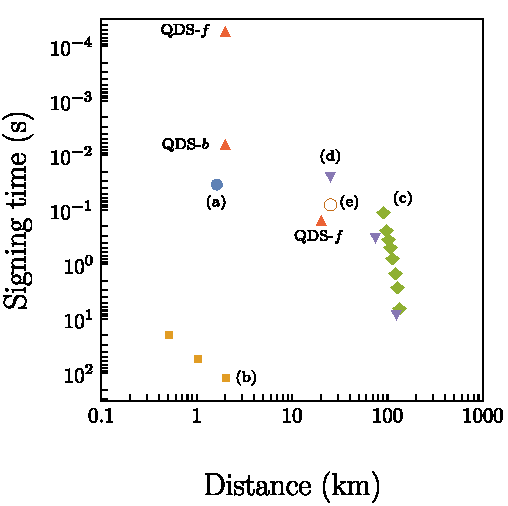
\includegraphics[width=1.0\linewidth, draft=false]{aqc/stargraph_ver2}
\caption{\label{fig:aqc_star} Time required to sign a one-bit message, and the corresponding channel lengths, for several recent QDS protocols. At the short distnaces ($\sim 2$~km) favoured by the continuous-variable platform, our QDS-$f$ and QDS-$b$ protocols allow for signing times of less than $0.05$~ms and $6$~ms, respectively, improving on previous results in CV (a) and discrete-variable (DV) (b) systems. At $20$~km, QDS-$f$ has a signing time comparable to recent DV QDS systems (c)-(e). Protocols depicted: red triangles - QDS-$b$ and QDS-$f$ from this chapter and Ref.~\cite{Richter2020}. (a) Free-space CV QDS \cite{Croal2016}. (b) Unambiguous-state-elimination-based QDS \cite{Donaldson2016}. (c) Differential-phase-shift-based QDS \cite{Collins2016}. (d) GHz BB$84$ QDS \cite{An2019}. (e) Early QDS-QKD ``agile'' system with measurement-device-independent capabilities \cite{Roberts2017}.}
\end{figure}


The calculated maximum secure key rates under protocol QKD-$f$ are plotted in Fig.~\ref{fig:aqc_qkdf} under attack BS$2$. The performance of this protocol agrees with Ref.~\cite{Papanastasiou2018} over comparable parameter regimes (when we analyse under the BS$0$ and EC attacks considered in that Paper), while the QPSK amplitudes employed in our experiment are much closer to optimal. Calculated maximum key rates, deduced from experimental parameters with models Sec.~\ref{sec:aqc_protocol_modifications}, are displayed in Tab.~\ref{tab:lengths}.

\begin{figure}[htp]
\centering
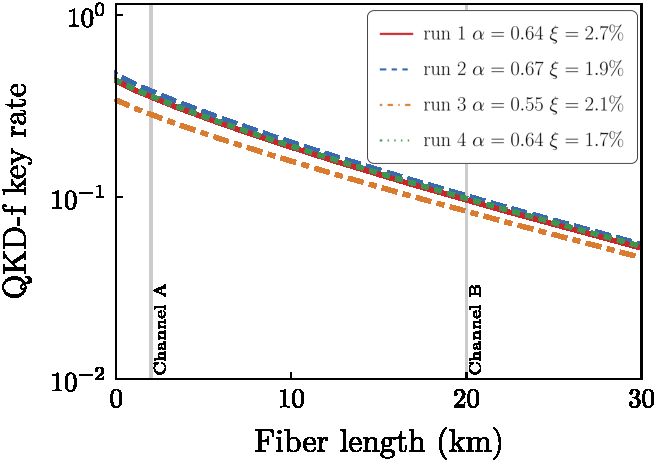
\includegraphics[width=0.8\linewidth, draft=false]{aqc/qkdf}
\caption{\label{fig:aqc_qkdf} Calculated maximum attainable key rates for protocol QKD-$f$. The predicted key rates agree with Ref.~\ref{Papanastasiou2018} over equivalent parameters, while the key rates displayed here are close to optimal. Vertical grid lines denote loss levels over experimental channels $A$ and $B$, corresponding to fiber lengths $2$~km ($0.65$~dB loss) and $20$~km ($4.75$~dB loss), respectively. Solid (red), dashed (blue), dot-dashed (orange) and dotted (green) lines correspond to experimental runs $1$, $2$, $3$ and $4$, respectively.}
\end{figure}



\clearpage
\section{Outlook}
We have observed efficient performance of each of our cryptographic protocols, QDS-$b$, QSS-$b$, QDS-$f$ and QKD-$f$, when key rates and signature lengths are estimated from the experimental data. Crucially, the experiment detailed in Sec.~\ref{sec:aqc_experiment} is performed without reference to any particular protocol and so the experimental hardware layer of Fig.~\ref{fig:big_agile} is agnostic to the application for which it is being used. Therefore, each system \systemB, \systemF \; may accurately be denoted ``agile''.

The clear separation of hardware layers from the software layer which selects the desired task is beneficial for practical implementation, and we believe that an agile middleware which enforces the separation will function analogously to the quantum compilers recently investigated in the context of quantum computing \cite{Killoran2018, qiskit, Murali2019}. Future quantum cryptographic protocols should be designed and optimized towards agility, and it should be possible to group additional existing cryptosystems into further agile systems for implementation.

The QDS protocols which we have investigated outperform their nearest competitors and allow for messages to be securely signed in (to our knowledge) the fastest observed times: less than $6$~ms for QDS-$b$ and less than $0.05$~ms for QDS-$f$. The trade-off of requiring short distances is not a huge one, since it has long been accepted \cite{Pirandola2015a} that continuous-variables cryptography boasting very high key rates and sending rates should be used for intra-city communication over distances the order of kilometers, while discrete-variables cryptography should be preferred for long-distance quantum communication. Moreover, our QSS-$b$ protocol is shown to require fewer quantum resources than an equivalent task accomplished via classical unconditionally secure secret sharing performed over pairwise encrypted QKD channels.

For our demonstrations, we have used experimental hardware which is almost entirely commercially available and is inherently compatible with existing classical communications infrastructure. In the future, this may render it possible to allow for quantum communications protocols to be performed over installed fibers with existing receivers, e.g. in the home, requiring merely an upgrade to their firmware. Our experiment was performed with a sending rate of $1$~GHz, but with similar hardware it is even possible to reach tens or hundreds of GHz \cite{Khan2015, Khan2016}, which would both improve the performance of our protocols, and make a practical eavesdropping attack increasingly difficult to perform. 

It is important to note that while the security techniques used here mirror the state-of-the-art techniques available for analysing e.g. QKD \cite{Papanastasiou2018} over similar setups, the requirement for QPSK states and heterodyne detection has proven restrictive to the amount of noise allowable on the channel under different attacks \cite{Zhao2009, Bradler2018}. Under EC attacks, protocols QDS-$f$, QSS-$b$ and QKD-$f$ remain insecure over the channels investigated, precisely because of the high level of excess noise $\xi$ which in a full treatment must be attributed to the eavesdropper. These protocols were therefore analysed in a ``trusted-noise" model, BS$2$, in which excess noise adversely affects honest players, but cannot be exploited by an eavesdropper. We believe that because of the high sending rates used in this experiment, and because of the the unknown (but assumed non-Gaussian) measurement which Eve performs in attack BS$2$, that the protocols still retain a high practical level of security, albeit technically not unconditional to all possible attacks. Future work should therefore endeavour to improve the security attainable for quantum cryptosystems relying on QPSK alphabet, and to improve the level of security proof for alphabets of coherent states modulated with a non-Gaussian distribution.

